\documentclass[unicode]{beamer}
\usepackage[utf8]{inputenc}
\usepackage[english,russian]{babel}
\usepackage{amsmath,amssymb}
\usepackage{epsfig}
\usepackage{graphicx}
\usepackage{hyperref}
\usepackage{appendixnumberbeamer}
%\usepackage[dvips]{color}


%\usepackage[compress]{beamerthemeMadrid}
%\usetheme{Warsaw}

\usetheme[numbers, totalnumbers, compress,nologo]{Statmod}
  %\setbeamercovered{transparent}


%\usepackage{beamerthemesplit}
%\usepackage{beamerthemeSingapore}
%\usepackage{beamerthemeJuanLesPins}
%\usepackage{beamerthemeMarburg}
%\usepackage{beamerthemePittsburgh}
%\usepackage{beamercolorthemecrane} %желтая тема
%\usepackage{beamercolorthemebeetle}
\usepackage{beamercolorthemeseagull} %cерая
%\usepackage{beamercolorthemefly} %на сером фоне
%\usepackage{beamercolorthemedove} %нет цветов
%\usepackage{beamercolorthemeseahorse}
%\usepackage{beamercolorthemerose}


\newcommand{\bhabha}{$e^+e^-$}
\newcommand{\erf}{\mbox{erf}}
\setbeamertemplate{sections/subsections in toc}[plain]

\newcommand{\ee}{e^{+}e^{-}}
\newcommand{\uu}{\mu^{+}\mu^{-}}
\newcommand{\KK}{K^{+}K^{-}}
\newcommand{\pipi}{\pi^{+}\pi^{-}}

\title{
	Измерение \vspace{1ex} \\
	$ \frac{B(J/\psi \to K^+K^-)}{B(J/\psi \to \mu^+\mu^-)}$ \\
\vspace{1ex}
с детектором BES-3}
\author{Николаев Иван}
\institute[ИЯФ СО РАН]
{ 
}

\begin{document}
\begin{frame}
  \maketitle
\end{frame}

\section{Введение}
\begin{frame}
\end{frame}
\section{Отбор событий}
\begin{frame}
\begin{enumerate}
	\item Ровно четыре заряженных трека из места встречи:
		\begin{itemize}
			\item Число заряженных треков $N_q = 4$
			\item Летят из места встречи: $|z| <  10$~см,  $r_{xy} < 1$~см. 
			\item На большие углы: $|\cos{\theta}|<0.8$
	  \end{itemize}

	\item Требуем ровно два разнозаряженных кандадата в пионы:
		\begin{itemize}
			\item $p(\pi^\pm) < 0.45$~ГэВ
			\item $3.0 < M_{rec}(\pipi)< 3.2$~ГэВ
		\end{itemize}

			\begin{figure}
			\begin{center}
			 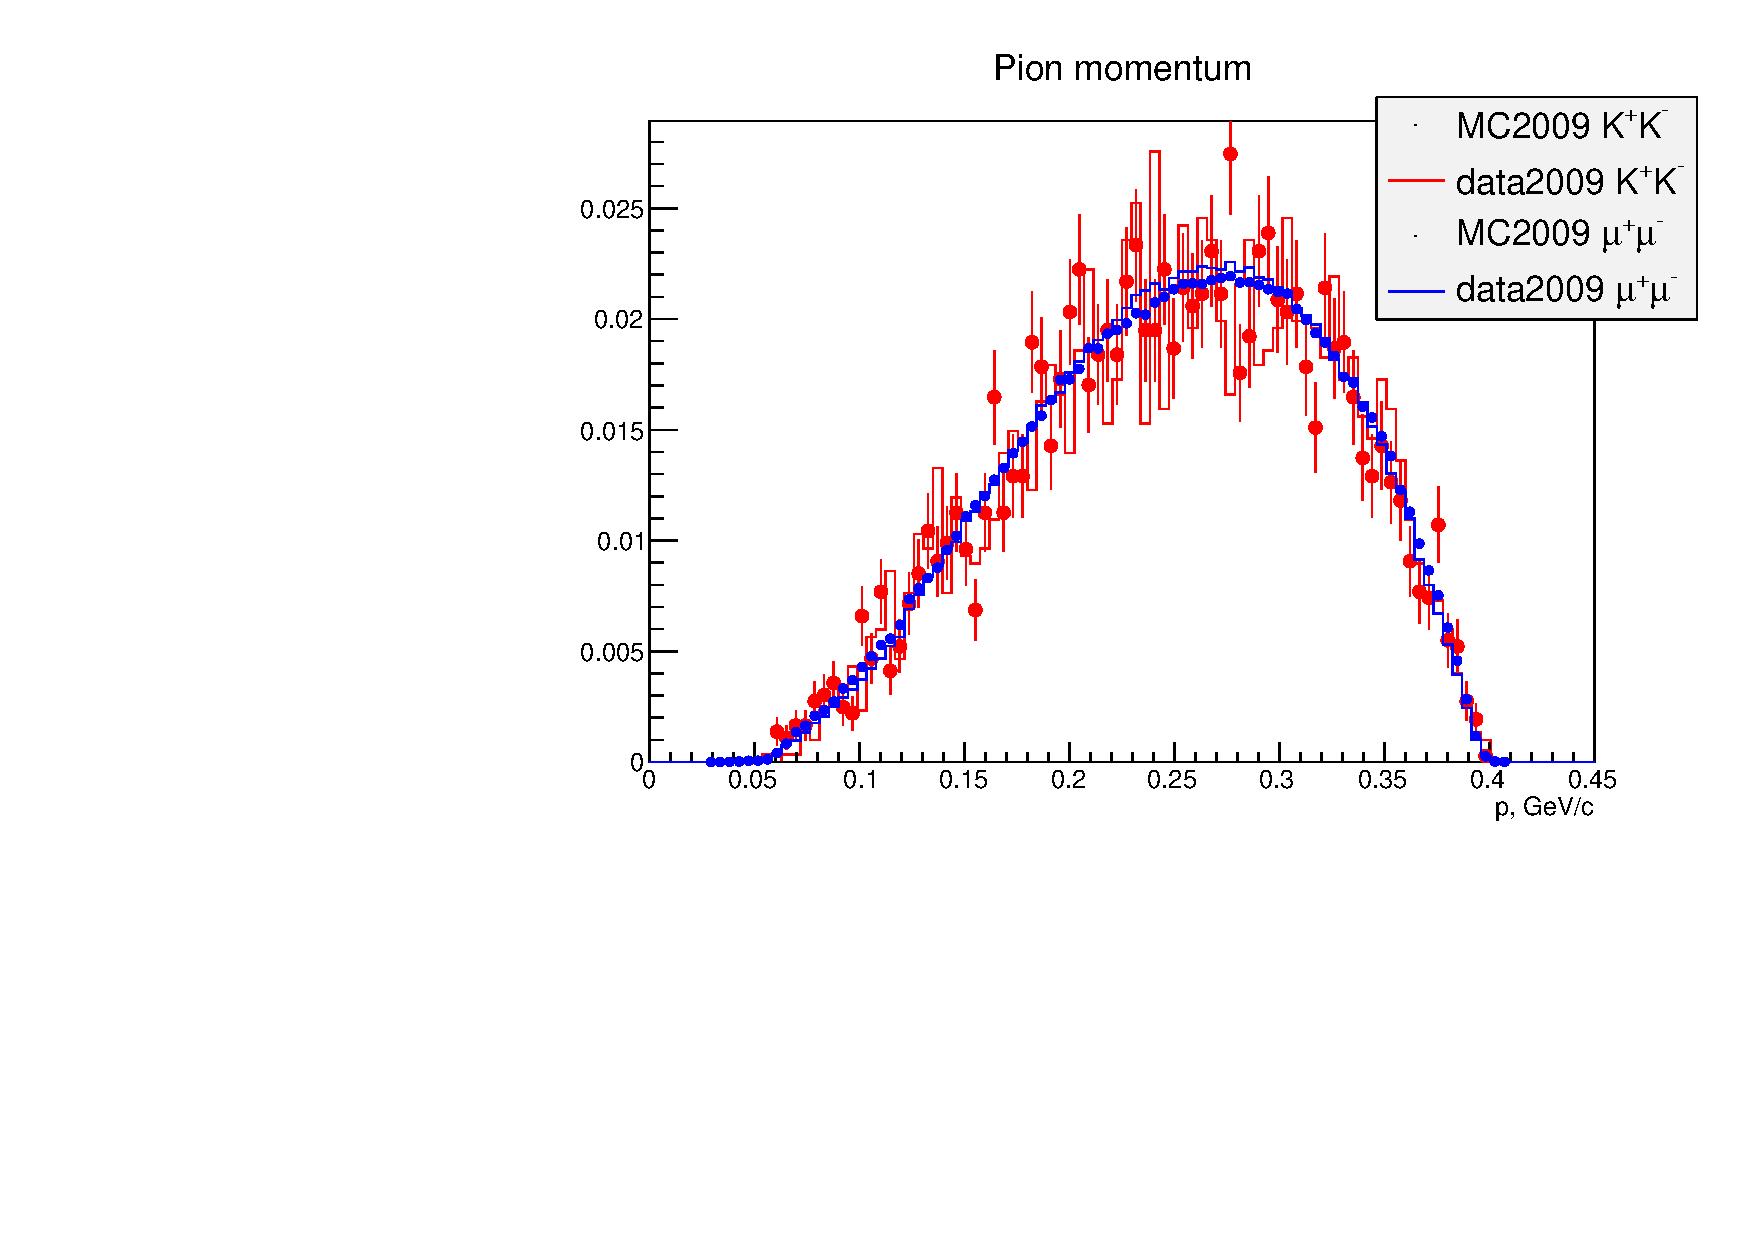
\includegraphics[width=0.45\textwidth]{fig/pion_momentum.pdf} \hfill
			 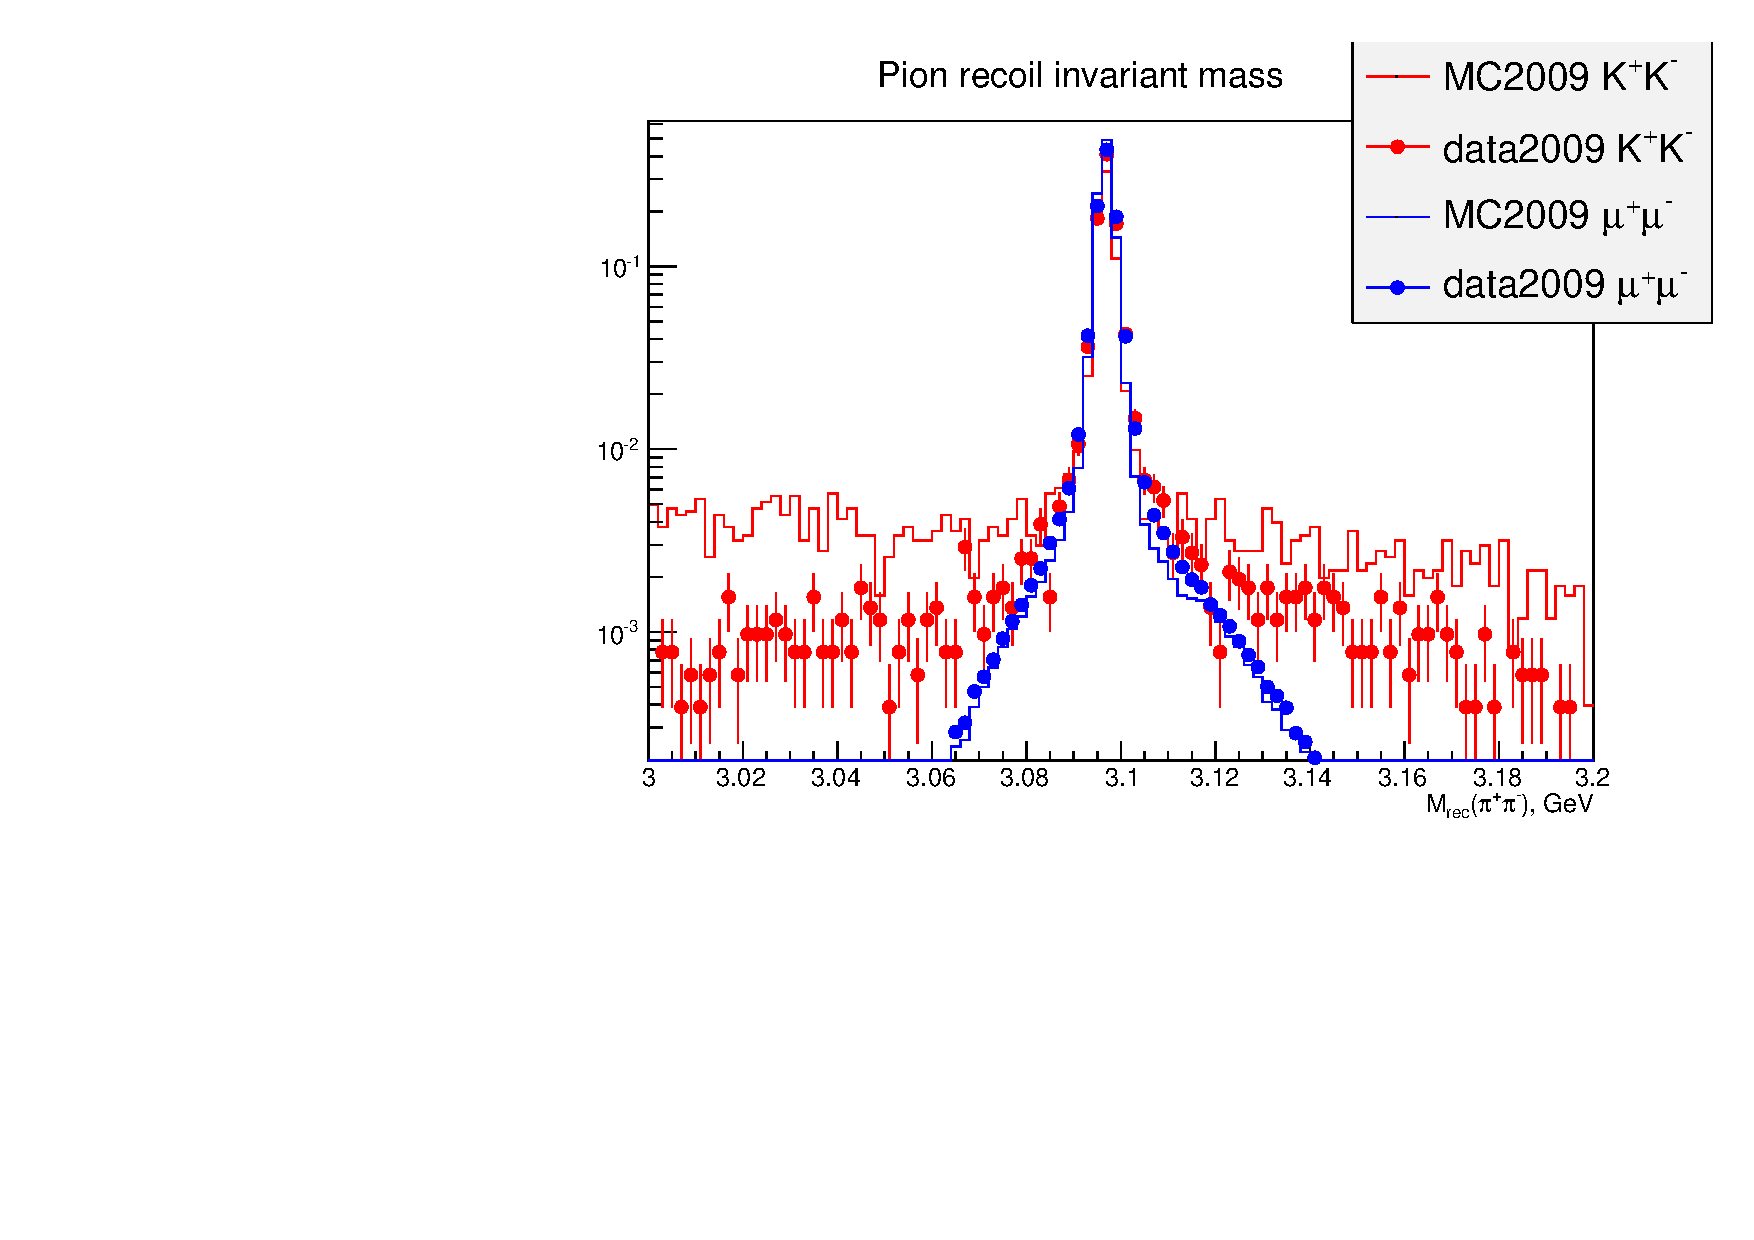
\includegraphics[width=0.45\textwidth]{fig/pion_Mrec.pdf}
			 %\caption{Pion momentum cut \mbox{$p<0.45$~GeV} is used. Pion recoil invariant mass cut $3.0 < M_{rec}(\pipi) < 3.2$~GeV is used}
			\end{center}
			\end{figure}
		\end{enumerate}
\end{frame}


\begin{frame}
	\begin{enumerate}
			\setcounter{enumi}{2}
	\item Остальные два разнозаряженных каон или мюон кандадаты:
		\begin{itemize}
			\item $1.0 < p(K^\pm, \mu^\pm ) < 2.0 $~ГэВ
			\item $E/p < 0.8$
		\end{itemize}
			\begin{figure}
			\begin{center}
				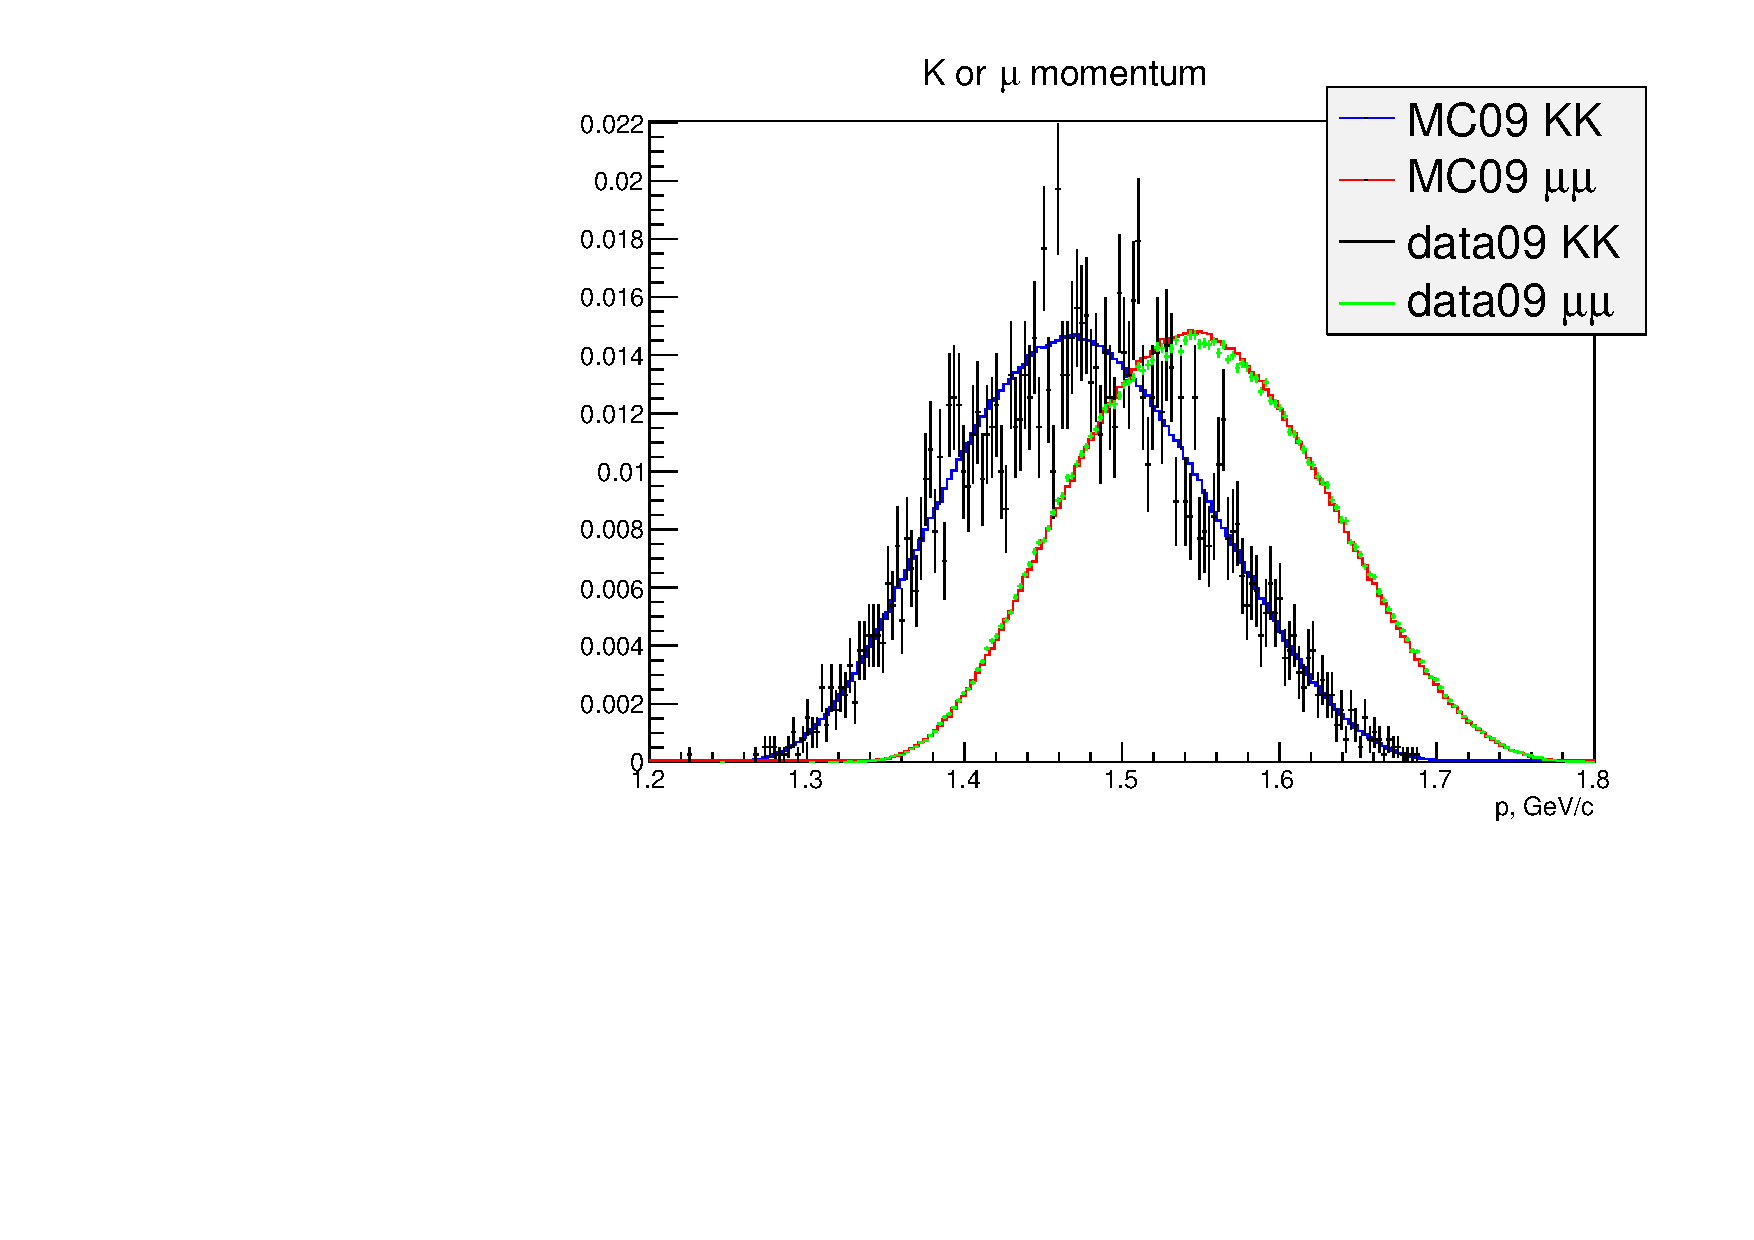
\includegraphics[width=0.45\textwidth]{fig/p.pdf} \hfill
				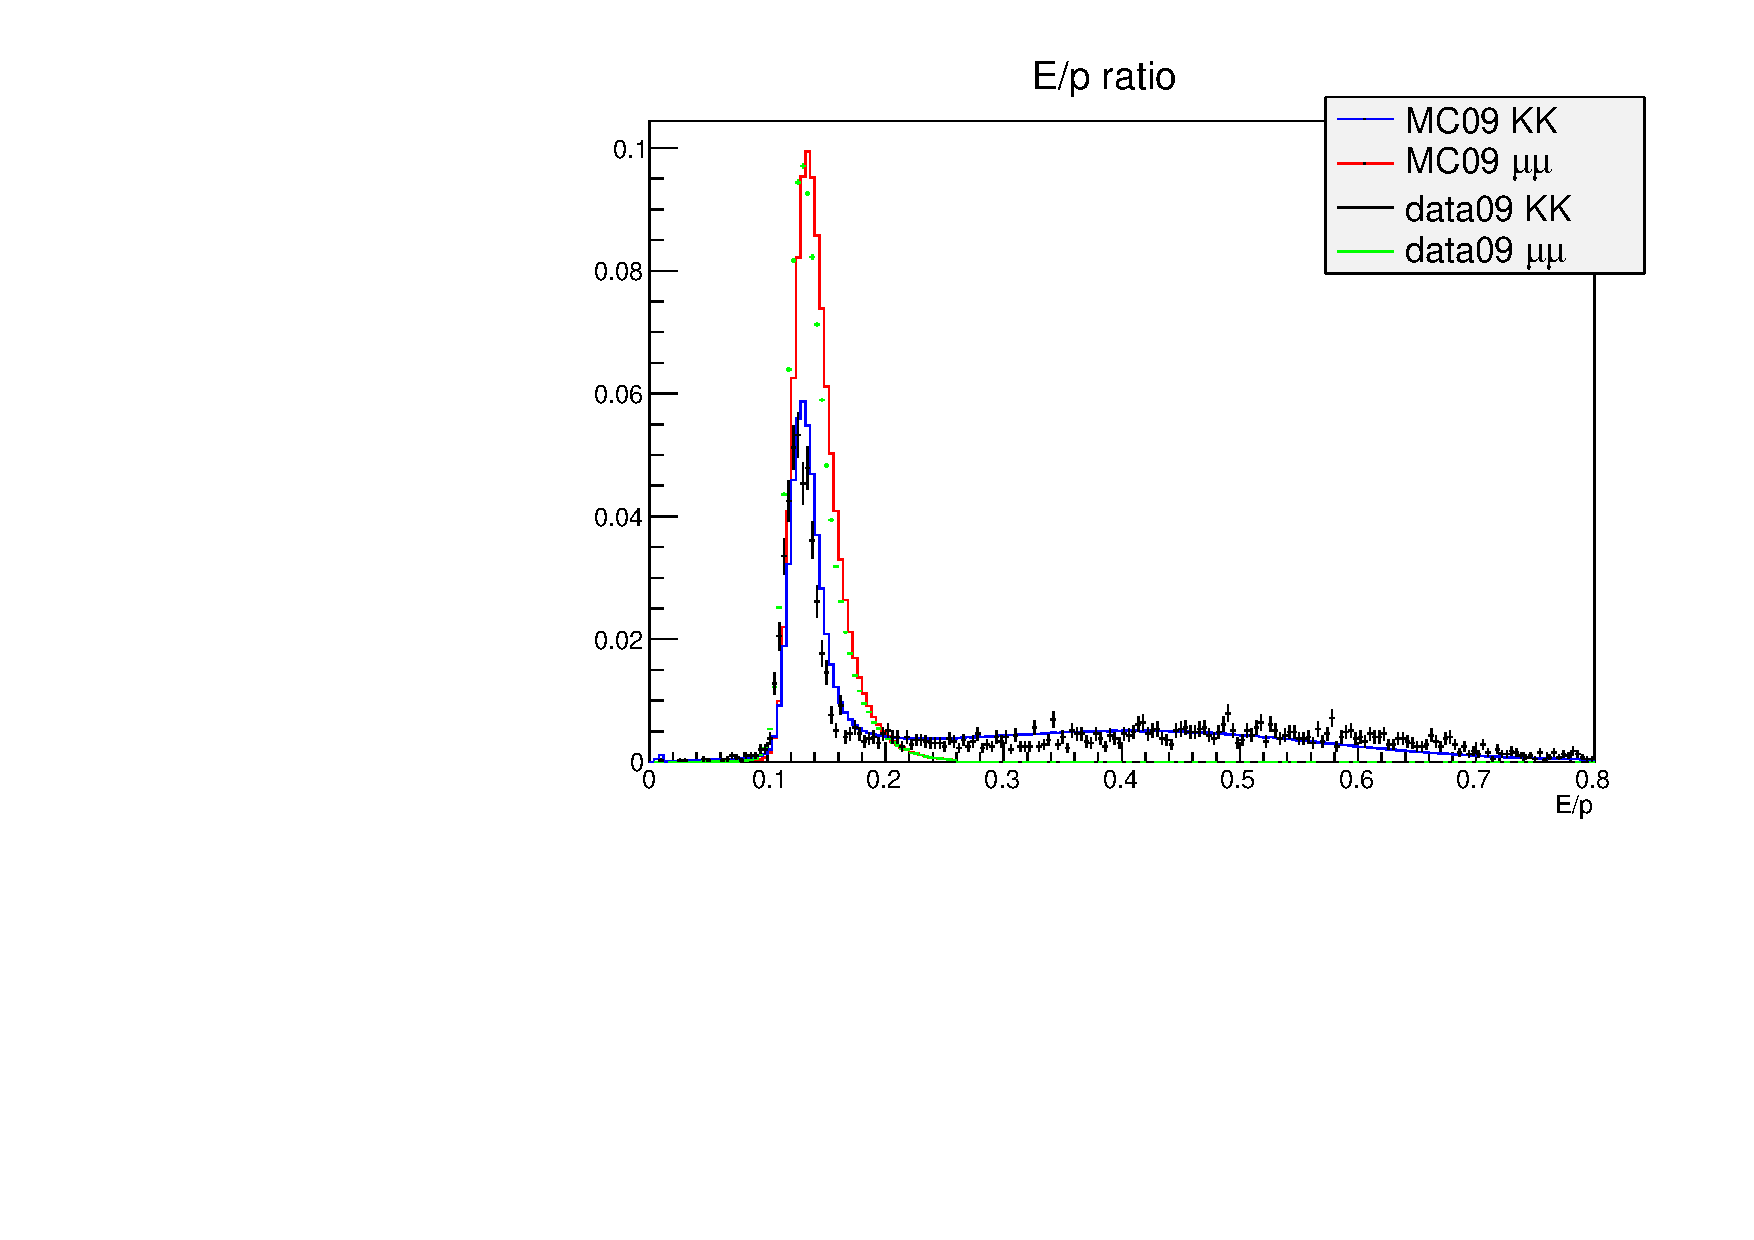
\includegraphics[width=0.45\textwidth]{fig/Ep.pdf}
			\end{center}
			\end{figure}

	\end{enumerate}
\end{frame}


\begin{frame}
	\begin{enumerate}
			\setcounter{enumi}{3}
	\item Кинематическая реконструкция по полному четырёхимпульсу с
		предварительным уточнением вершины в гипотезе мюонов или каонов.
		\begin{itemize}
			\item $\chi^2_{kin}(KK) < 40$
			\item $\chi^2_{kin}(\mu\mu) < 40$
		\end{itemize}
		\item Идентификация по $dE/dx$ и  $TOF$;
			\renewcommand{\arraystretch}{1.8}
			\begin{itemize}
				\item $\chi^2_{pid}(pid) = \sum\limits_{track}^{}\chi^2_{dEdx}(pid) + \chi^2_{TOF}(pid)$
				\item $\chi^2_{pid}(KK) < 20$
				\item $\chi^2_{pid}(\mu\mu) < 20$
				\end{itemize}

			\begin{figure}
			\begin{center}
				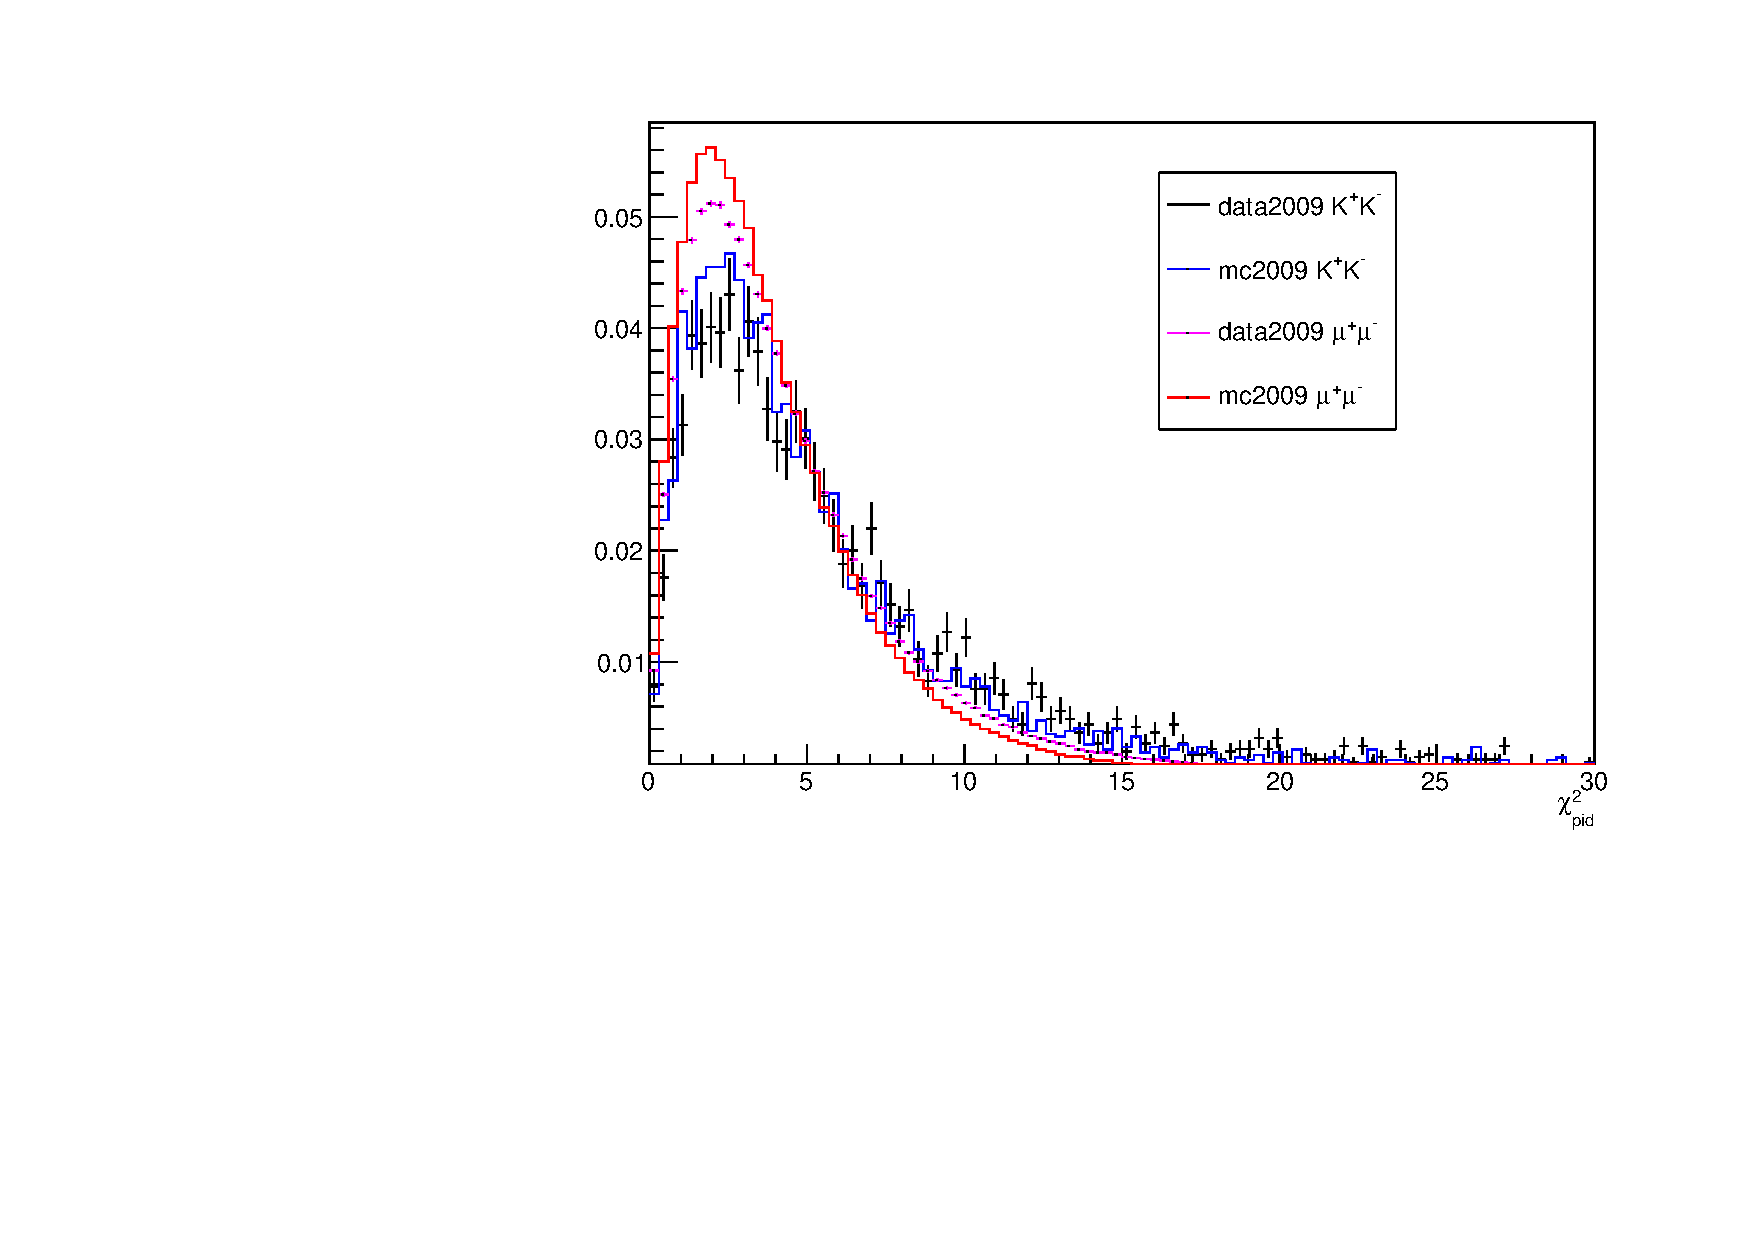
\includegraphics[width=0.45\textwidth]{fig/pid_chi2-09.pdf} \hfill
				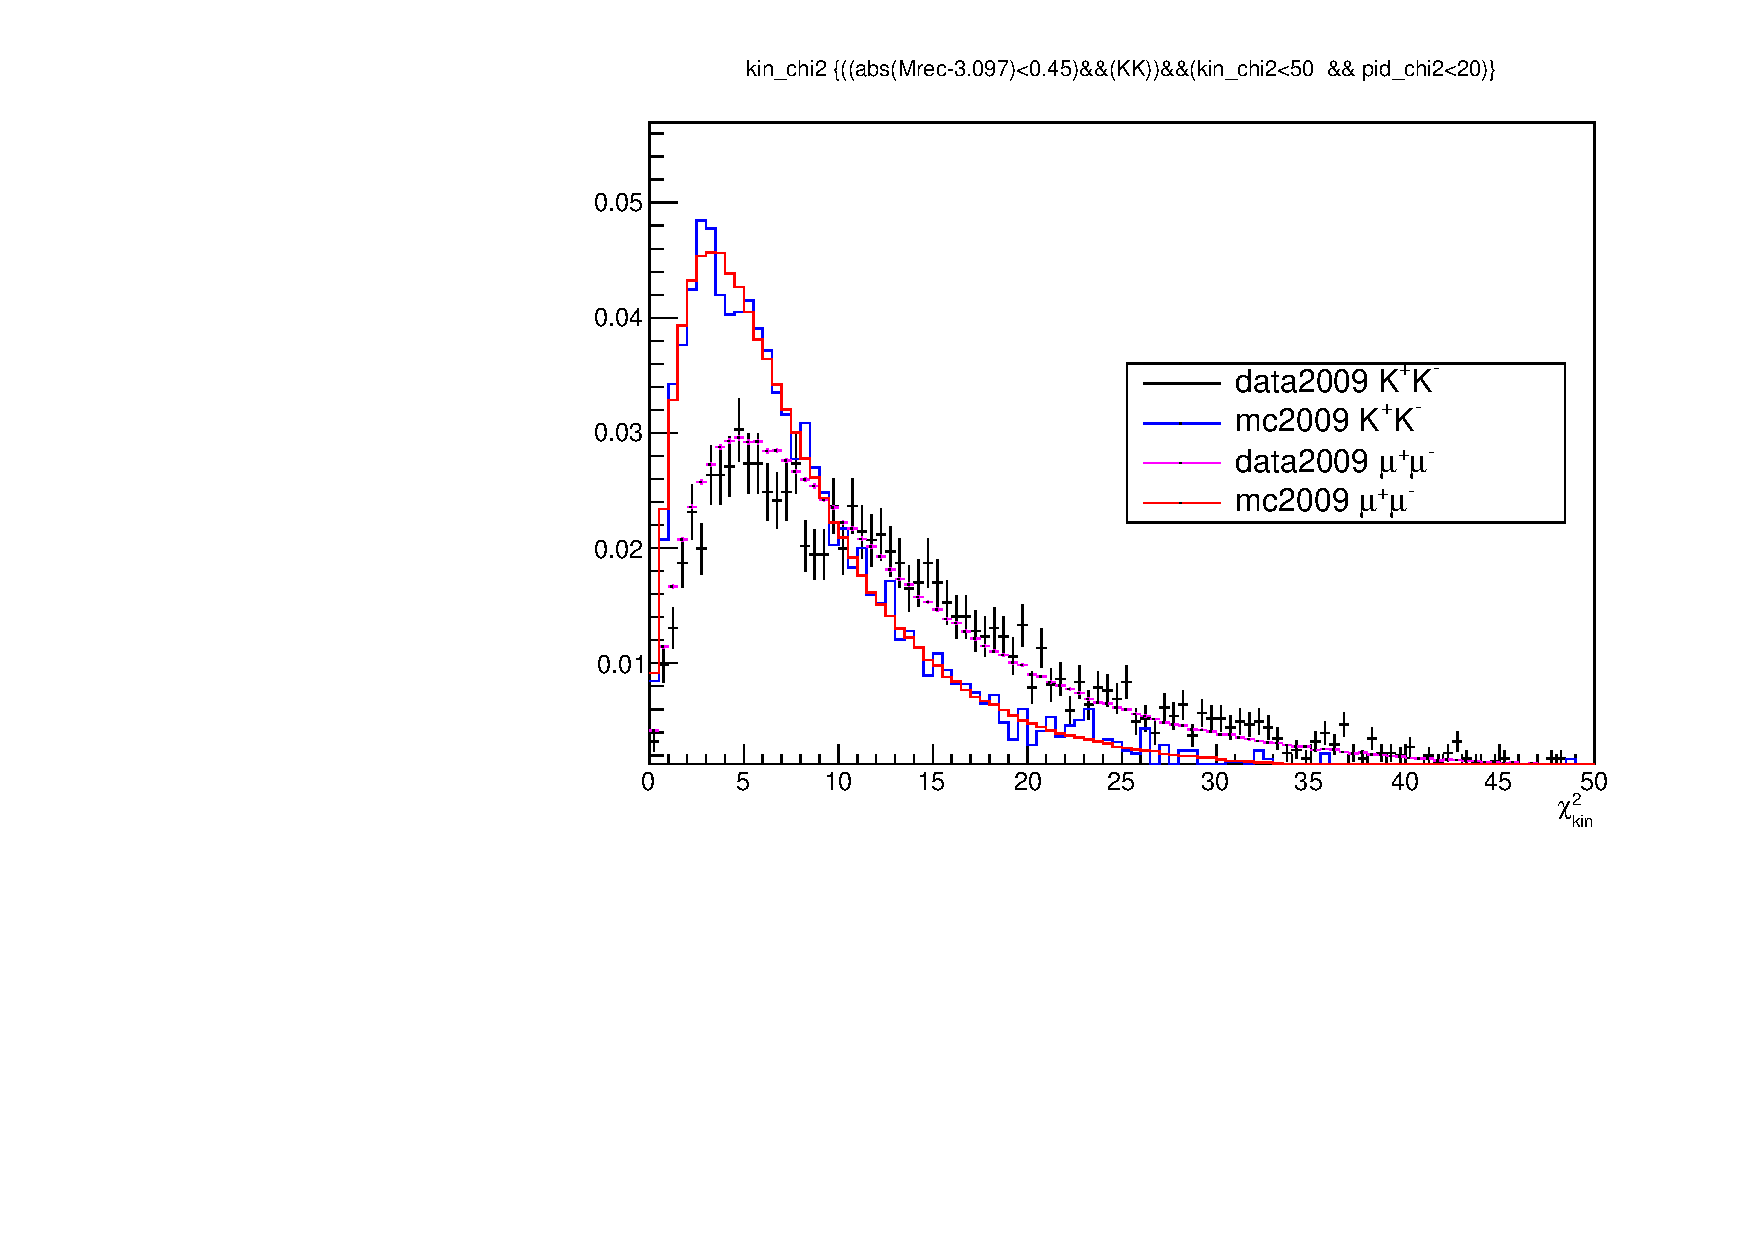
\includegraphics[width=0.45\textwidth]{fig/kin_chi2-09.pdf}
			\end{center}
			\end{figure}
		\end{enumerate}

\end{frame}


\begin{frame}
	\begin{enumerate}
			\setcounter{enumi}{5}
		\item Разделение $\uu$,  $\KK$: \\
			\begin{minipage}{0.45\textwidth}
			 Случай $\uu$:
				\begin{itemize}
					\item $\chi_{kin}^2(\mu\mu) < \chi_{kin}^2(KK)$
					\item $\chi_{pid}^2(\mu\mu) < \chi_{pid}^2(KK)$
					\item $E/p < 0.8$
				\end{itemize}
			\end{minipage}
			\hfill
			\begin{minipage}{0.45\textwidth}
	 Случай $\uu$:
		\begin{itemize}
			\item $\chi_{kin}^2(\mu\mu) < \chi_{kin}^2(KK)$
			\item $\chi_{pid}^2(\mu\mu) < \chi_{pid}^2(KK)$
			\item $E/p < 0.26$
		\end{itemize}
			\end{minipage}
	\end{enumerate}
\end{frame}

\section{Анализ фона}
\begin{frame}
	\frametitle{Фоны}
	\begin{itemize}
		\item Пучковый
		\item Космика
		\item Распады $\psi(2S)$
		\item Континуум
	\end{itemize}
\end{frame}
\begin{frame}
\tiny
\frametitle{Inclusive Monte Carlo 2009, $KK$-channel}
 \begin{table}
   \centering
   \begin{tabular}{rrcl} \\
\#    &   count & final state & decay topology                      \\   \hline   
  1   &       1 & $\pi\pi \mu\mu$ & $  \psi(2S) \to \pipi (J/\psi \to \uu)                       $ \\ 
	2   &       2 & $\pi\pi KK$ & $  \psi(2S) \to (\bar K^*(892)^0 \to \pi^+ K-)(K_0^*(1430)^0 \to \pi^-K^+) +c.c.  $ \\ 
  3   &       2 & $\pi\pi KK$ & $  \psi(2S) \to (\rho(770)^0 \to \pipi )\KK                    $ \\ 
  4   &       2 & $\pi\pi KK$ & $  \psi(2S) \to \pi^+K^-(K_2^*(1430)^0 \to \pi^-K^+)     +c.c.          $ \\ 
  5   &      14 & $\pi\pi KK$ & $  \psi(2S) \to (\bar K^*(892)^0 \to \pi^+ K^-)(K_2^*(1430)^0 \to \pi^-K^+) +c.c.  $ \\ 
  6   &      24 & $\pi\pi KK$ & $  \psi(2S) \to (K^*(892)^0 \to \pi^-K^+)(\bar K^*(892)^0 \to \pi^+ K^-)   $ \\ 
  7   &      25 & $\pi\pi KK$ & $  \psi(2S) \to \pipi \KK                                $ \\ 
  8   &      27 & $\pi\pi KK$ & $  \psi(2S) \to K^-(K_1(1270)^+ \to (\rho(770)^0 \to \pipi )K^+)+c.c.    $ \\ 
  9   &      53 & $\pi\pi KK$ & $  \psi(2S) \to K^-(K_1(1270)^+ \to \pipi K^+)      +c.c.          $ \\ 
 10   &      73 & $\pi\pi KK$ & $  \psi(2S) \to \pi^+K^-(K^*(892)^0 \to \pi^- K^+)   +c.c.             $ \\ 
 11   &     112 & $\pi\pi KK$ & $  \psi(2S) \to K^-(K_1(1270)^+ \to \pi^+ (K^*(892)^0 \to \pi^-K^+))   +c.c. $ \\ 
 12   &     248 & $\pi\pi KK$ & $  \psi(2S) \to K^-(K_1(1270)^+ \to \pi^+ (K_0^*(1430)^0 \to \pi^- K^+)) +c.c.$ \\ 
 13   &    2801 & $\pi\pi KK$ & $  \psi(2S) \to \pipi (J/\psi \to \KK )                       $ \\ \hline
 \end{tabular}
 \end{table}

\begin{figure}
	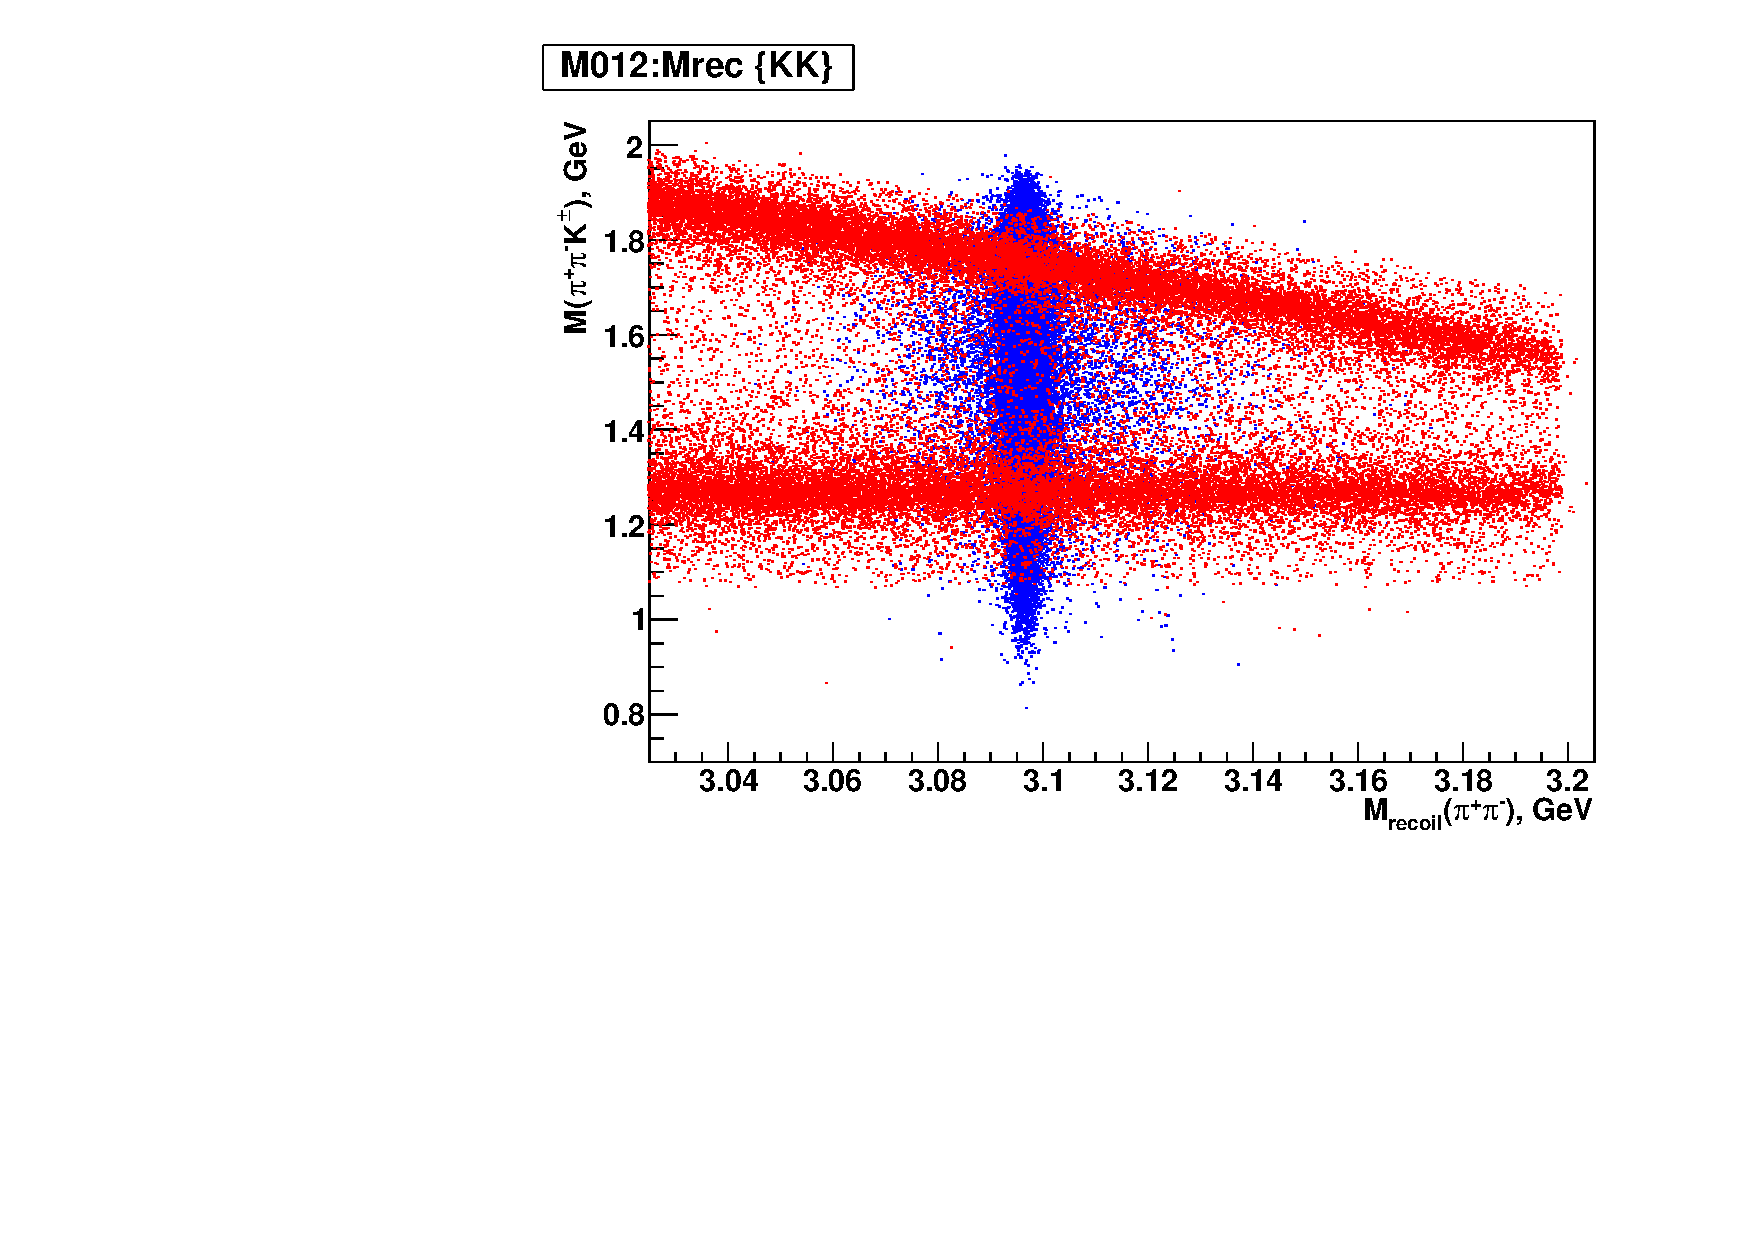
\includegraphics[width=0.4\textwidth]{fig/M012_Mrec-color.pdf} \hfill
%	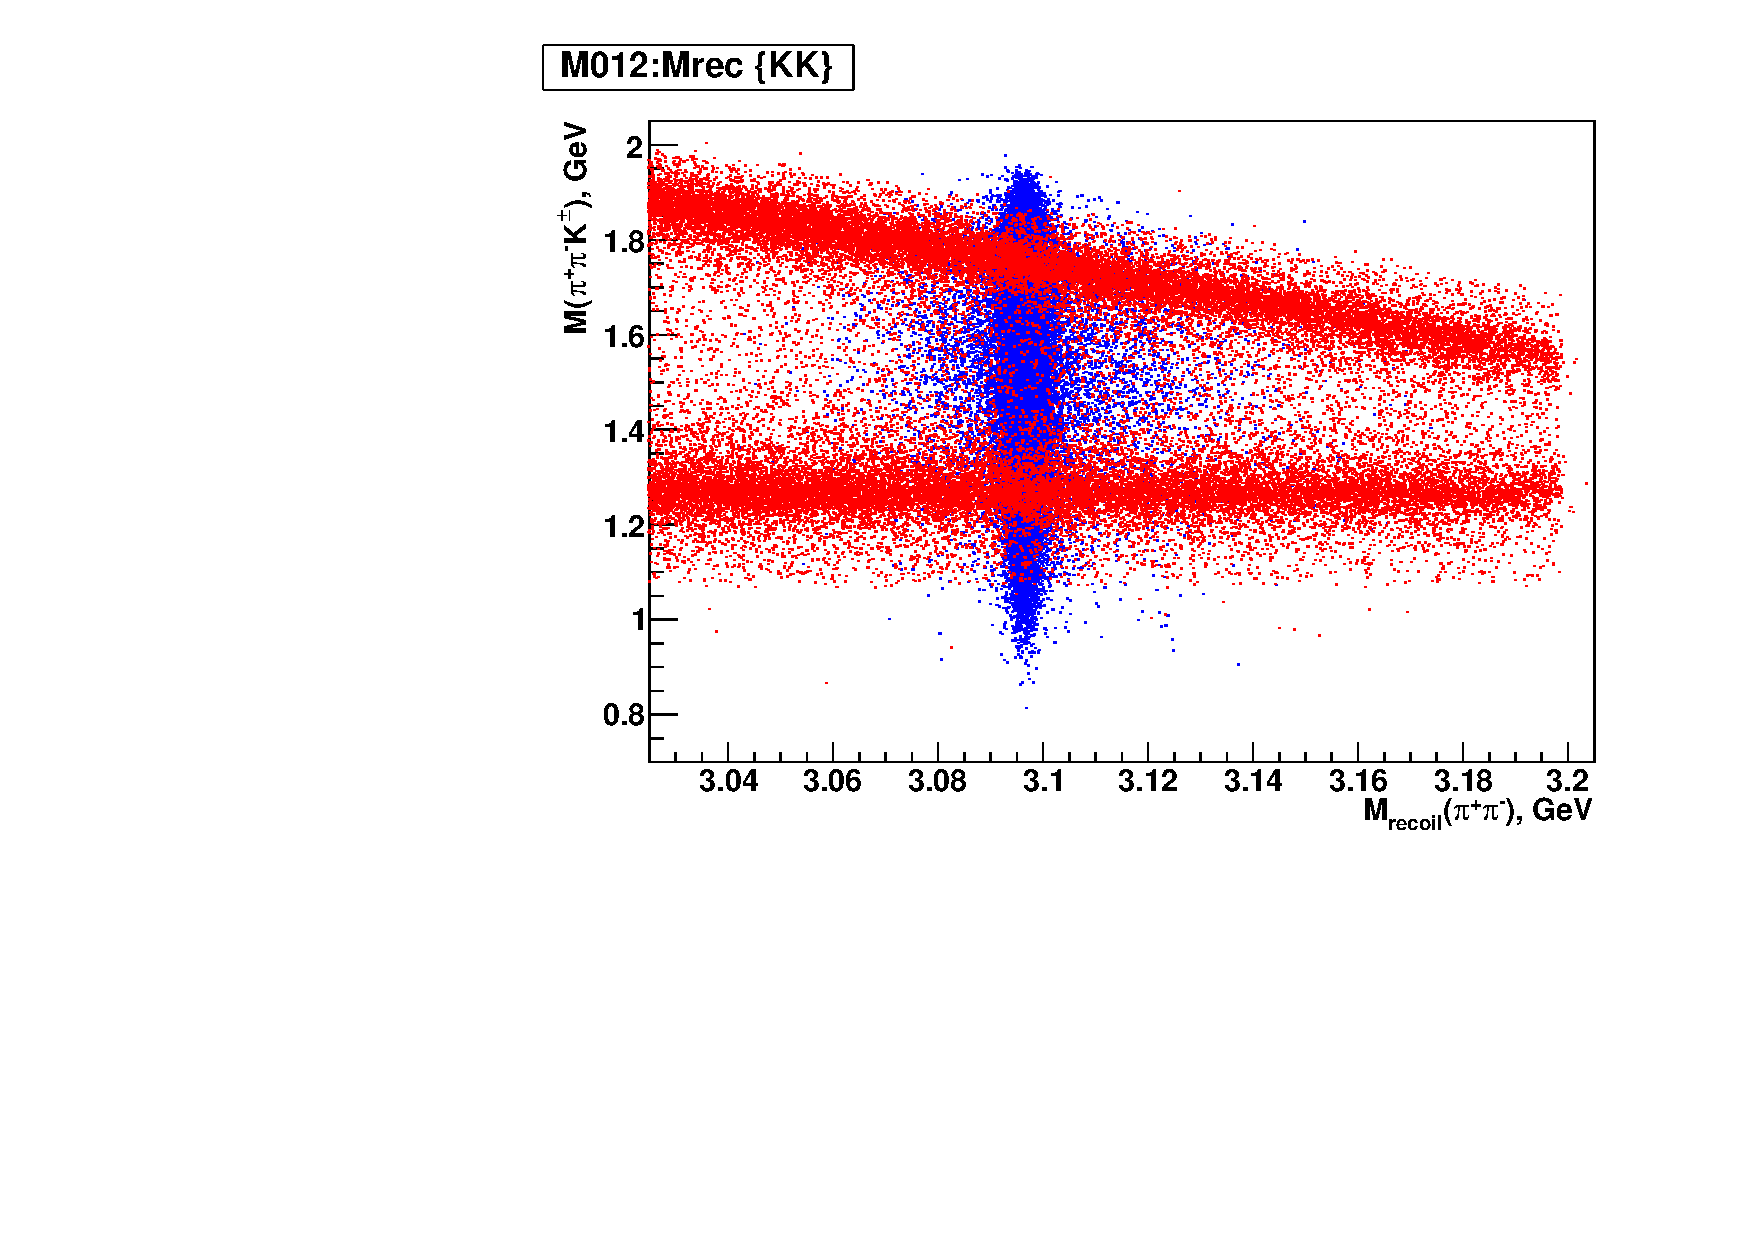
\includegraphics[width=0.4\textwidth]{fig/M012_Mrec-color.pdf} \hfill
\end{figure}
\end{frame}


\begin{frame}
   \frametitle{Inclusive Monte Carlo 2009, $\mu\mu$-channel}
	 \tiny \begin{table}
   \centering
   \label{tab:KKtopo}
   \begin{tabular}{rrrl} \\
  \#   &  count & final state & decay topology                      \\   \hline   
  1&        1 &$ \gamma\pi\pi\pi\pi        $ &$ \psi(2S) \to \pipi(J/\psi \to \gamma(f_2(1270) \to \pipi))       $\\ 
  2&        1 &$ ee\mu\mu\gamma\gamma\gamma$ &$ \psi(2S) \to (\pi_0 \to \ee\gamma)(\pi_0 \to \gamma\gamma)(J/\psi \to \uu)    $\\ 
  3&        1 &$ \mu\mu\mu\mu\gamma        $ &$ \psi(2S) \to (\eta \to \uu\gamma)(J/\psi \to \uu)              $\\ 
  4&        1 &$ \pi\pi\pi\pi              $ &$ \psi(2S) \to \pipi\pipi                           $\\ 
  5&        1 &$ ee\mu\mu\gamma            $ &$ \psi(2S) \to (\eta \to \ee\gamma)(J/\psi \to \uu)              $\\ 
  6&        1 &$ \gamma\pi\pi\pi\pi        $ &$ \psi(2S) \to \pipi(J/\psi \to \gamma(f_2(2150) \to \pipi))       $\\ 
  7&        2 &$ \pi\pi\pi\pi              $ &$ \psi(2S) \to \pi^+(b_1(1235)^- \to \pi^-(\omega(782) \to \pipi)) +c.c.   $\\ 
  8&        2 &$ \mu\mu                    $ &$ \psi(2S) \to \uu                                 $\\ 
  9&        3 &$ \pi\pi\pi\pi              $ &$ \psi(2S) \to \pi^-(a_2(1320)^+ \to (\rho(770)^0 \to \pipi)\pi^+) +c.c.  $\\ 
 10&        5 &$ \gamma\pi\pi\pi\pi        $ &$ \psi(2S) \to \pipi(J/\psi \to \gamma(f_4(2050) \to \pipi))       $\\ 
 11&       13 &$ \pi\pi\pi\pi              $ &$ \psi(2S) \to (\rho(770)^0 \to \pipi)\pipi                 $\\ 
 12&       77 &$ \mu\mu\gamma \pi\pi       $ &$ \psi(2S) \to (\eta \to \gamma\pipi)(J/\psi \to \uu)              $\\ 
 13&      589 &$ \pi\pi\pi\pi              $ &$ \psi(2S) \to \pipi(J/\psi \to \pipi)                     $\\ 
 14&   675597 &$ \mu\mu\pi\pi              $ &$ \psi(2S) \to \pipi(J/\psi \to \uu)                     $\\ \hline
 \end{tabular}
 \end{table}
 \begin{itemize}
	 \item Доля фона: 697/675597 = 0.1\%
	 \end{itemize}
\end{frame}


\section{Fit to recoil mass}
\begin{frame}
	\frametitle{Fit to recoil mass: Modified double Crystal Ball function }
\begin{equation}
	f_{CB}(x)  = 	\left\{
		\begin{array}{lrrr}
			D_l e^{\kappa_l x},  &         -\infty   &   x < & -\gamma_l \\
			A_l(B_l - x)^{-n_l},  & -\gamma_l &   x <&   -\alpha_l \\
			A_{el}\exp(\alpha_{el}x), &  -\alpha_l & < x  < &-\alpha_{el} \\
			\exp( - x^2/2),  &  - \alpha_{el} & < x < & \alpha_{er} \\
			A_{er}\exp(-\alpha_{er}x), &  \alpha_{el} & < x < & -\alpha_{r} \\
			A_r(B_r + x)^{-n_r}, &   \alpha_r & < x < & \gamma_r \\
			D_r e^{-\kappa_r x},  &            &   x < & \infty
		\end{array}
		\right., 
\end{equation}
\begin{equation}
	\begin{array}{lcl}
		A_{er, el} & = &  \exp(\alpha_{er, el}^2/2) \\
		B_{ r, l}  &  = & n_{r, l}/ \alpha_{er, el} - \alpha_{r, l} \\
		D_{r, l}   &  = &  \frac{A_{r, l} e^{\kappa_{r, l}\gamma_{r, l}}}{(B_{r, l} + \gamma_{r, l})^{n_{r, l}}}
	\end{array}
\end{equation}
\end{frame}

\begin{frame}
	\begin{block}{\small Mote Carlo 2009}
\begin{figure}
	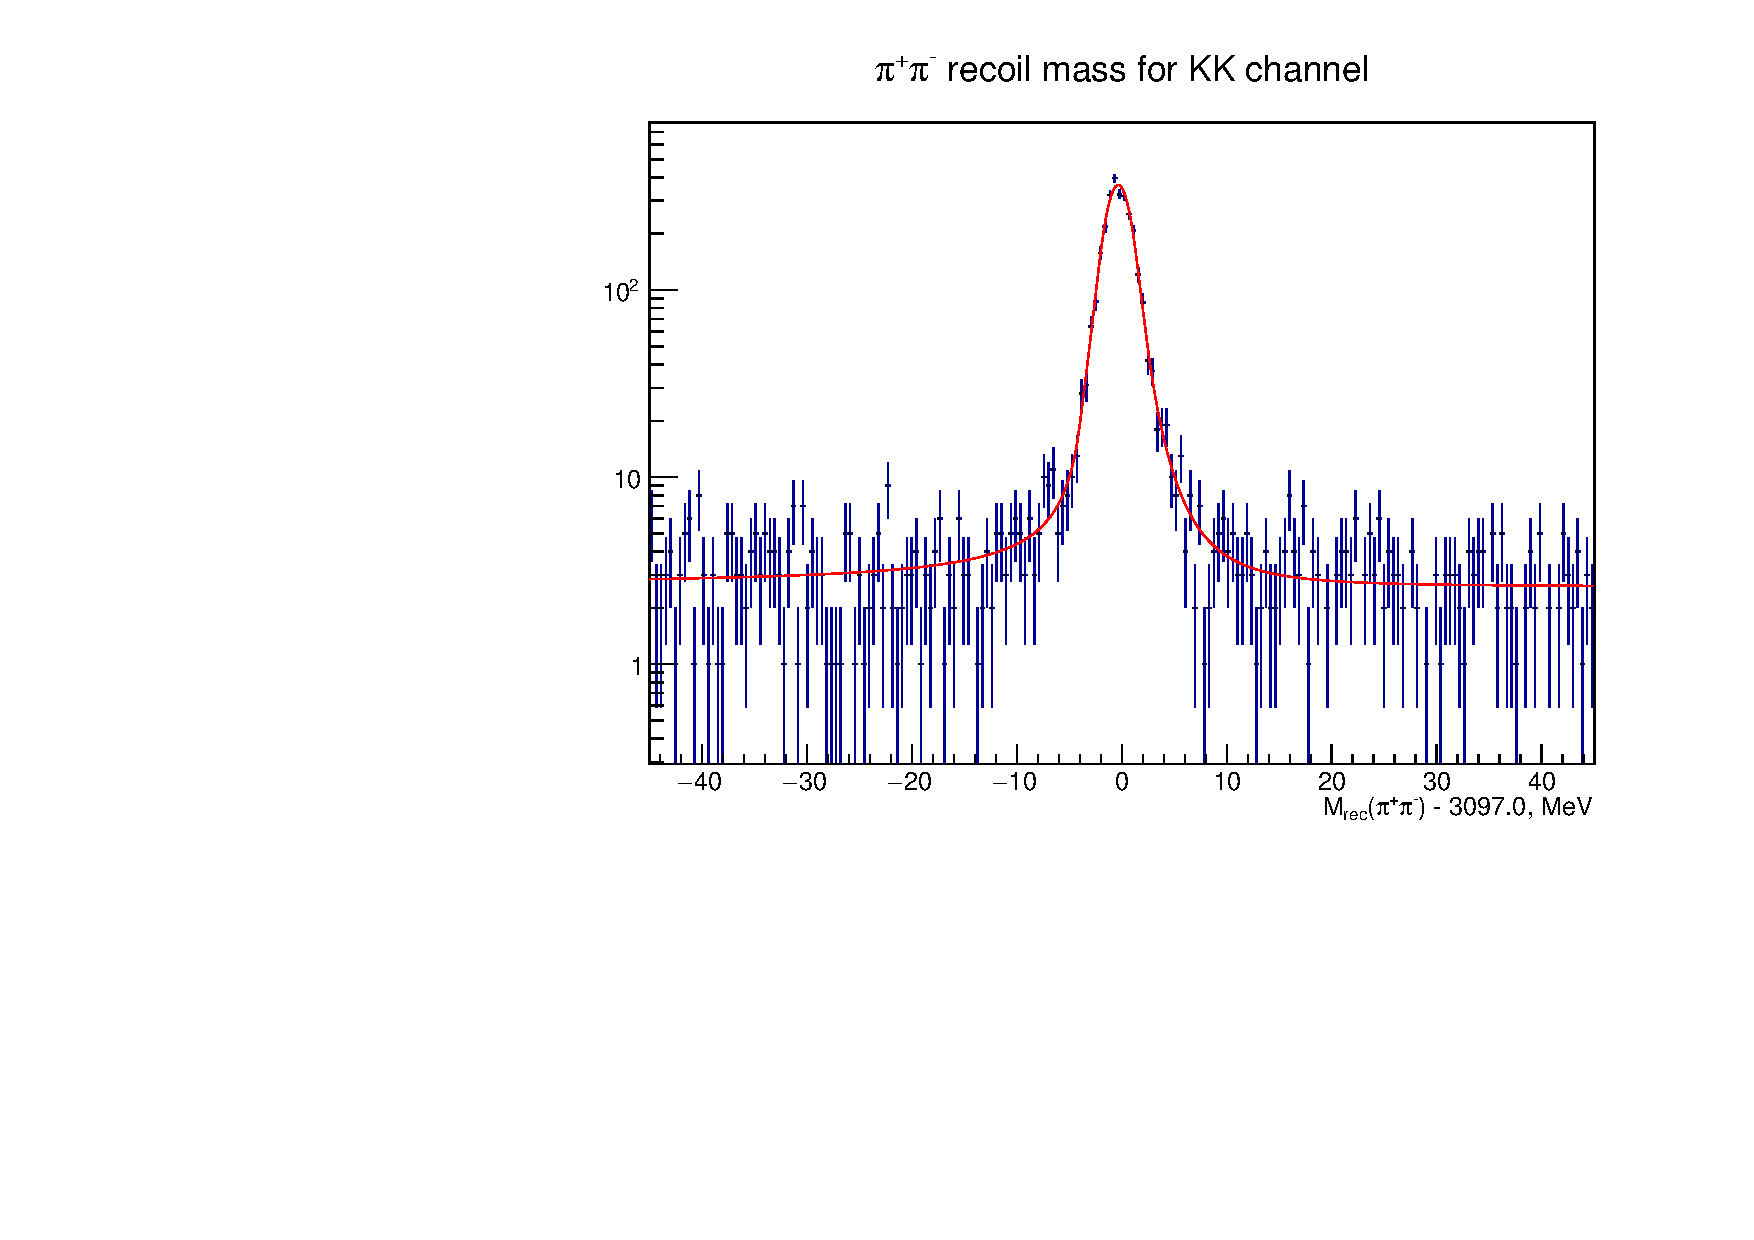
\includegraphics[width=0.45\textwidth]{fig/MrecKK09.pdf} \hfill
	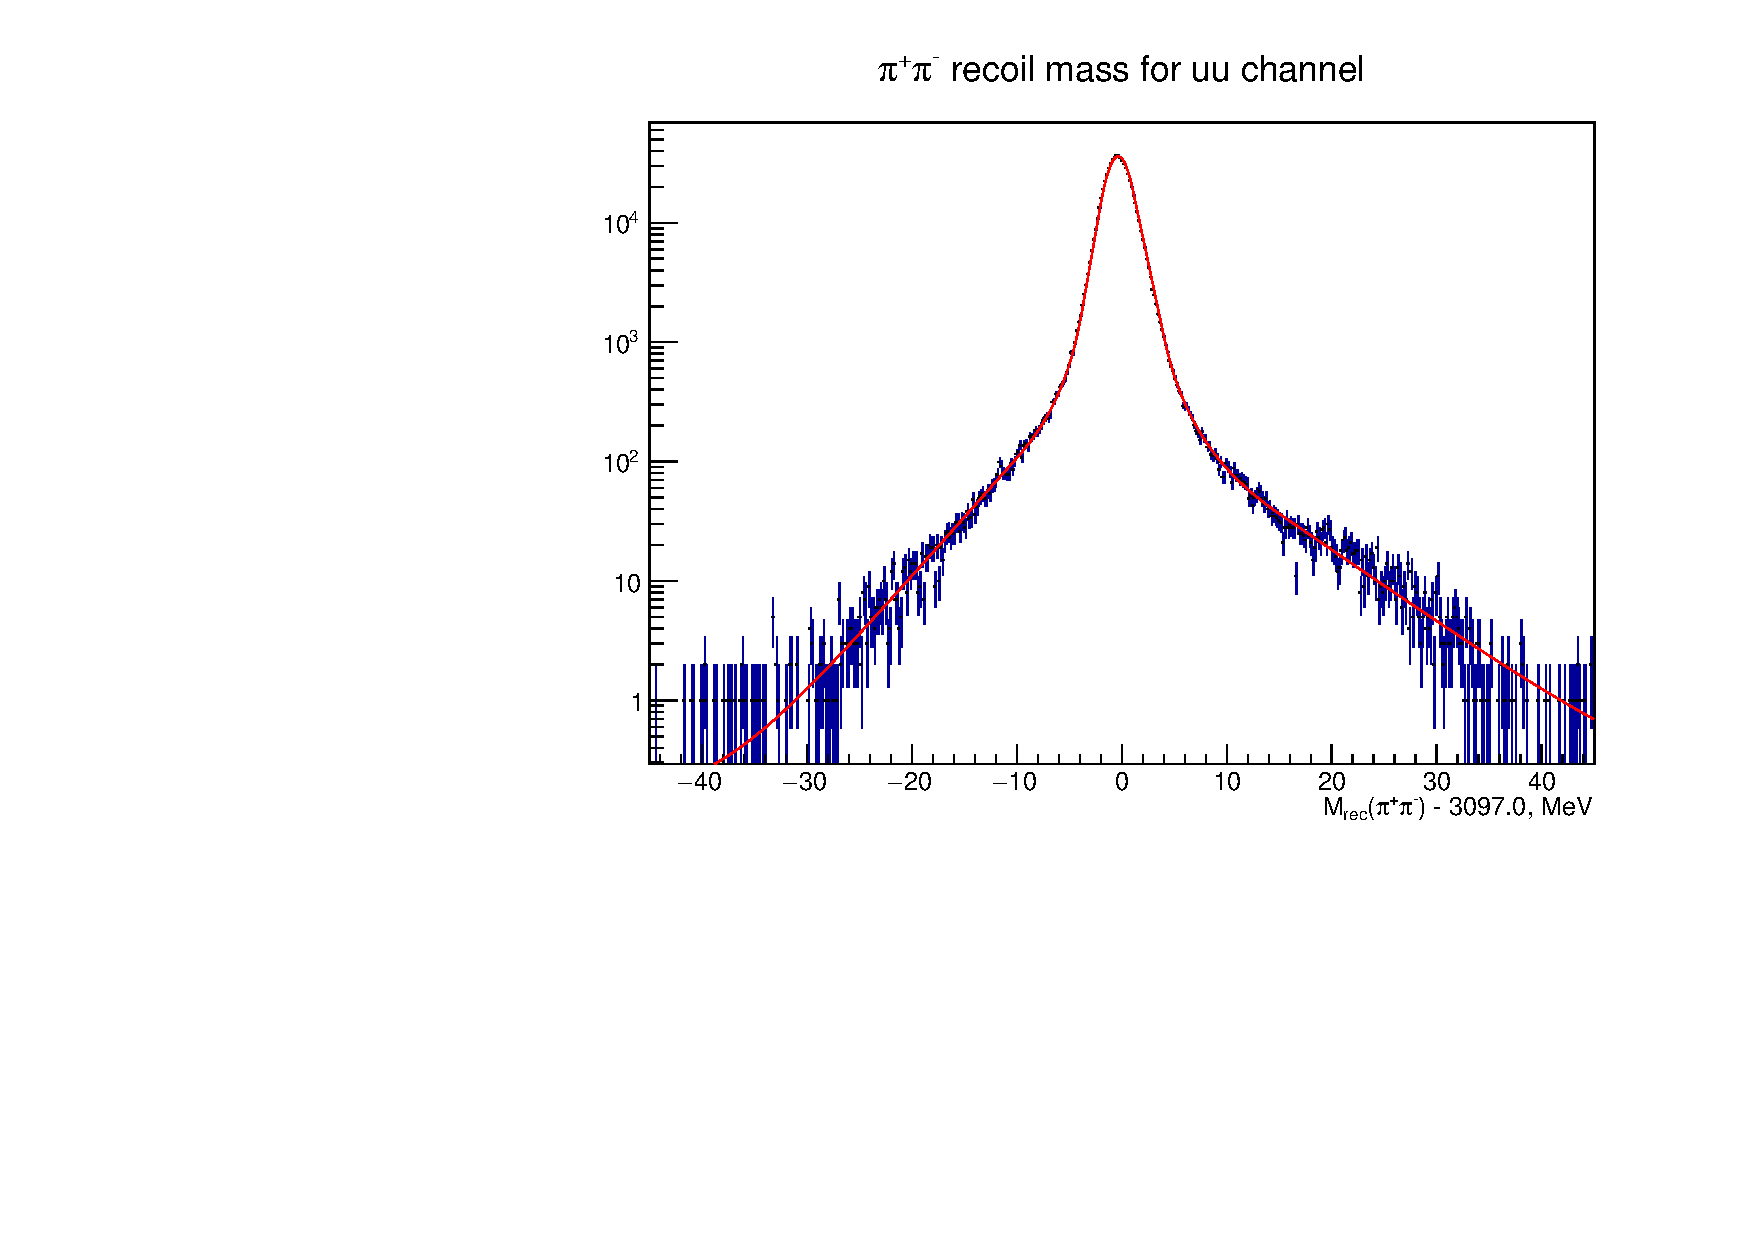
\includegraphics[width=0.45\textwidth]{fig/MrecUU09.pdf} \hfill
\end{figure}
\end{block}
	\begin{block}{\small Data 2009}
\begin{figure}
	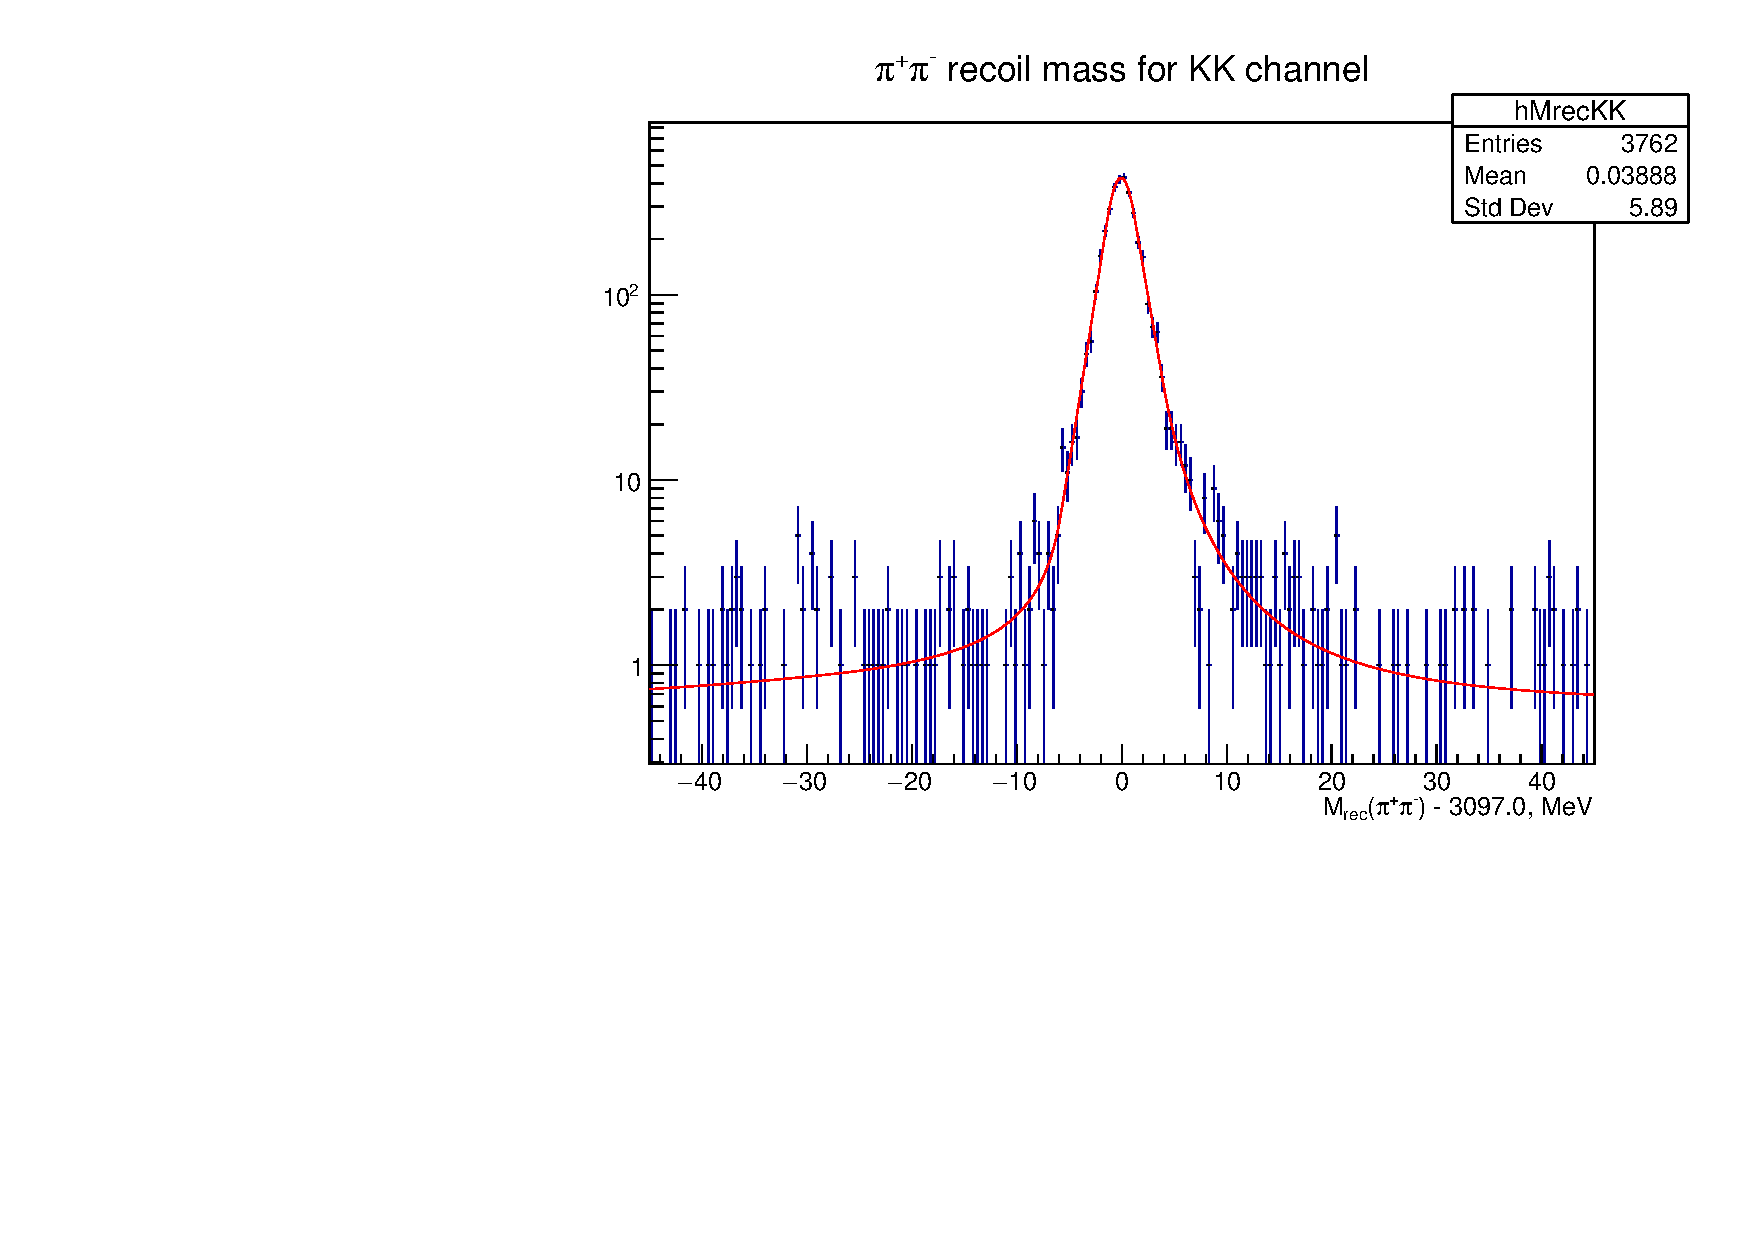
\includegraphics[width=0.45\textwidth]{fig/data09-MrecKK.pdf} \hfill
	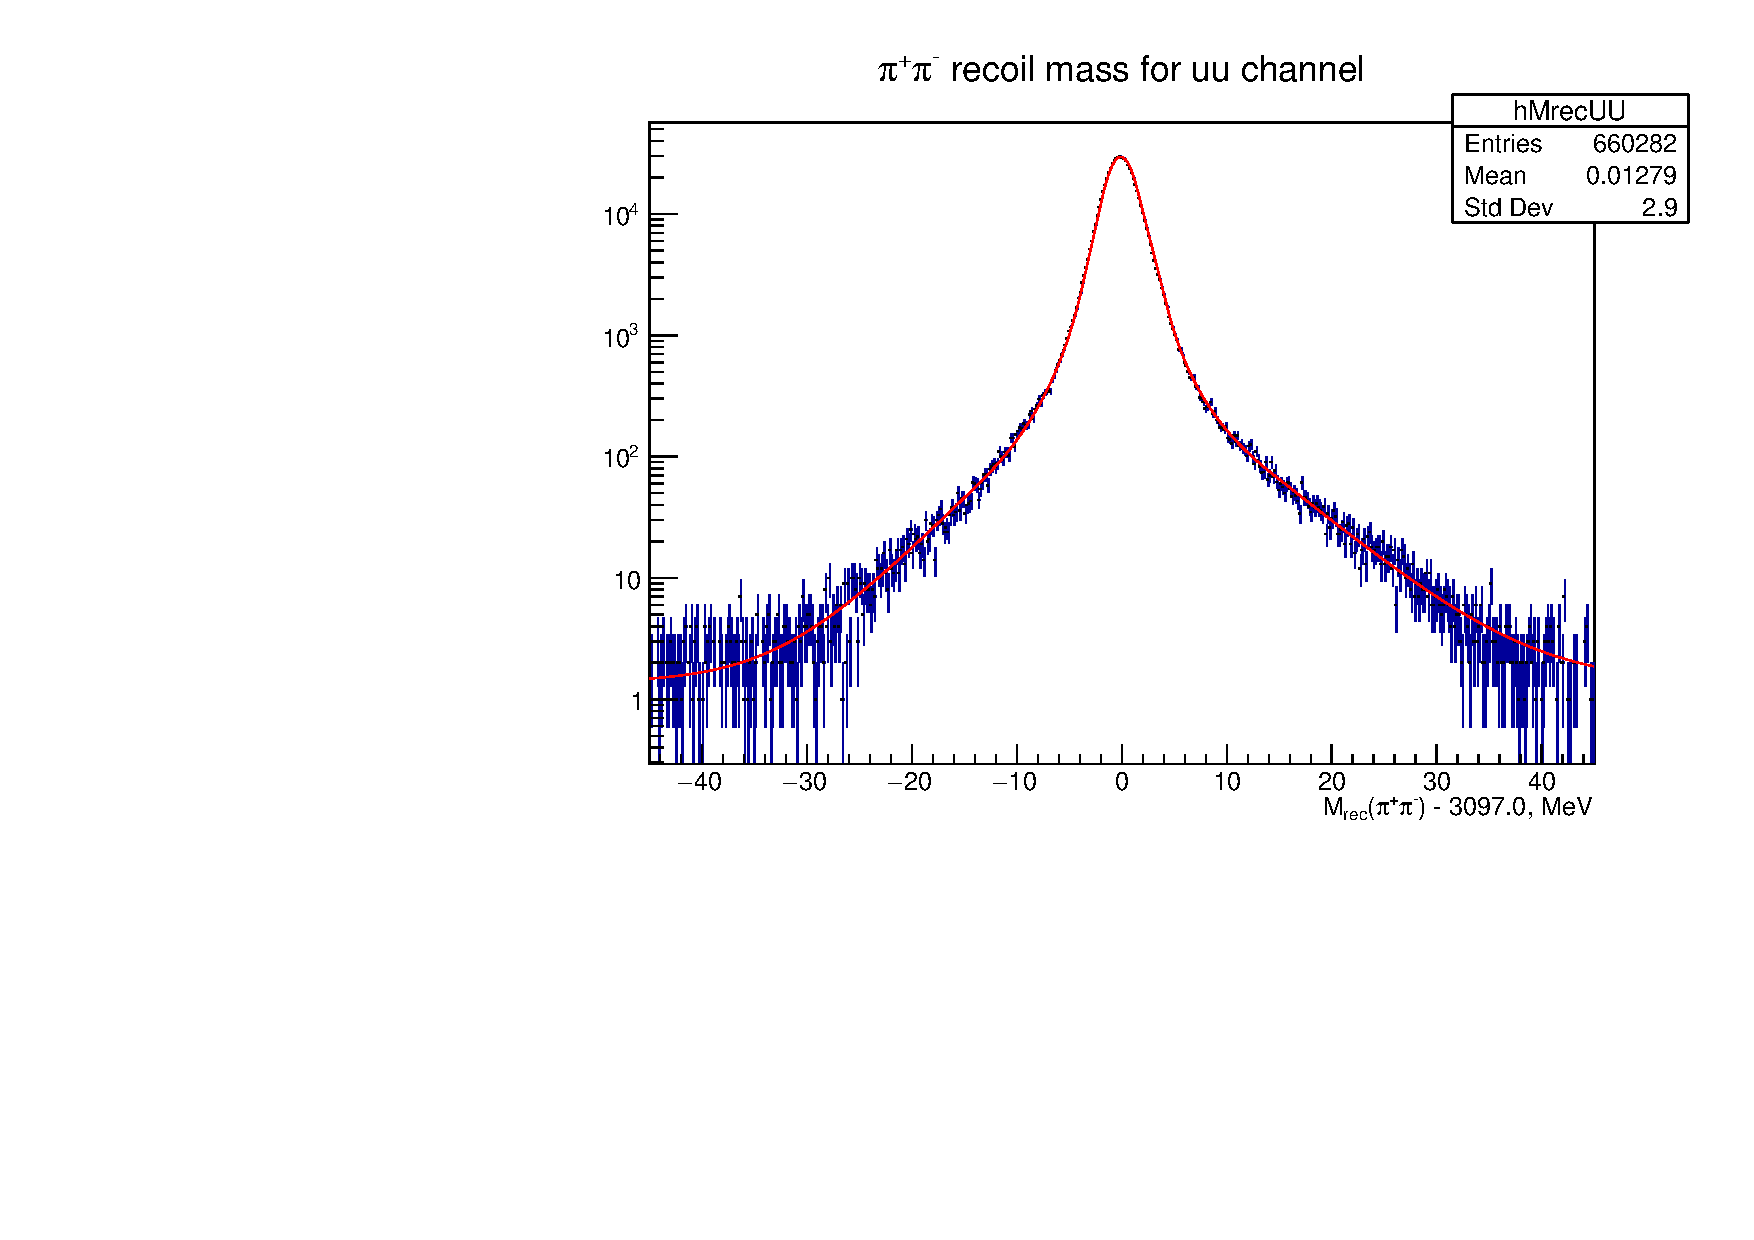
\includegraphics[width=0.45\textwidth]{fig/data09-MrecUU.pdf} \hfill
\end{figure}
\end{block}
\end{frame}
\begin{frame}
	
	\begin{block}{Радиационные фотоны}
\begin{figure}
	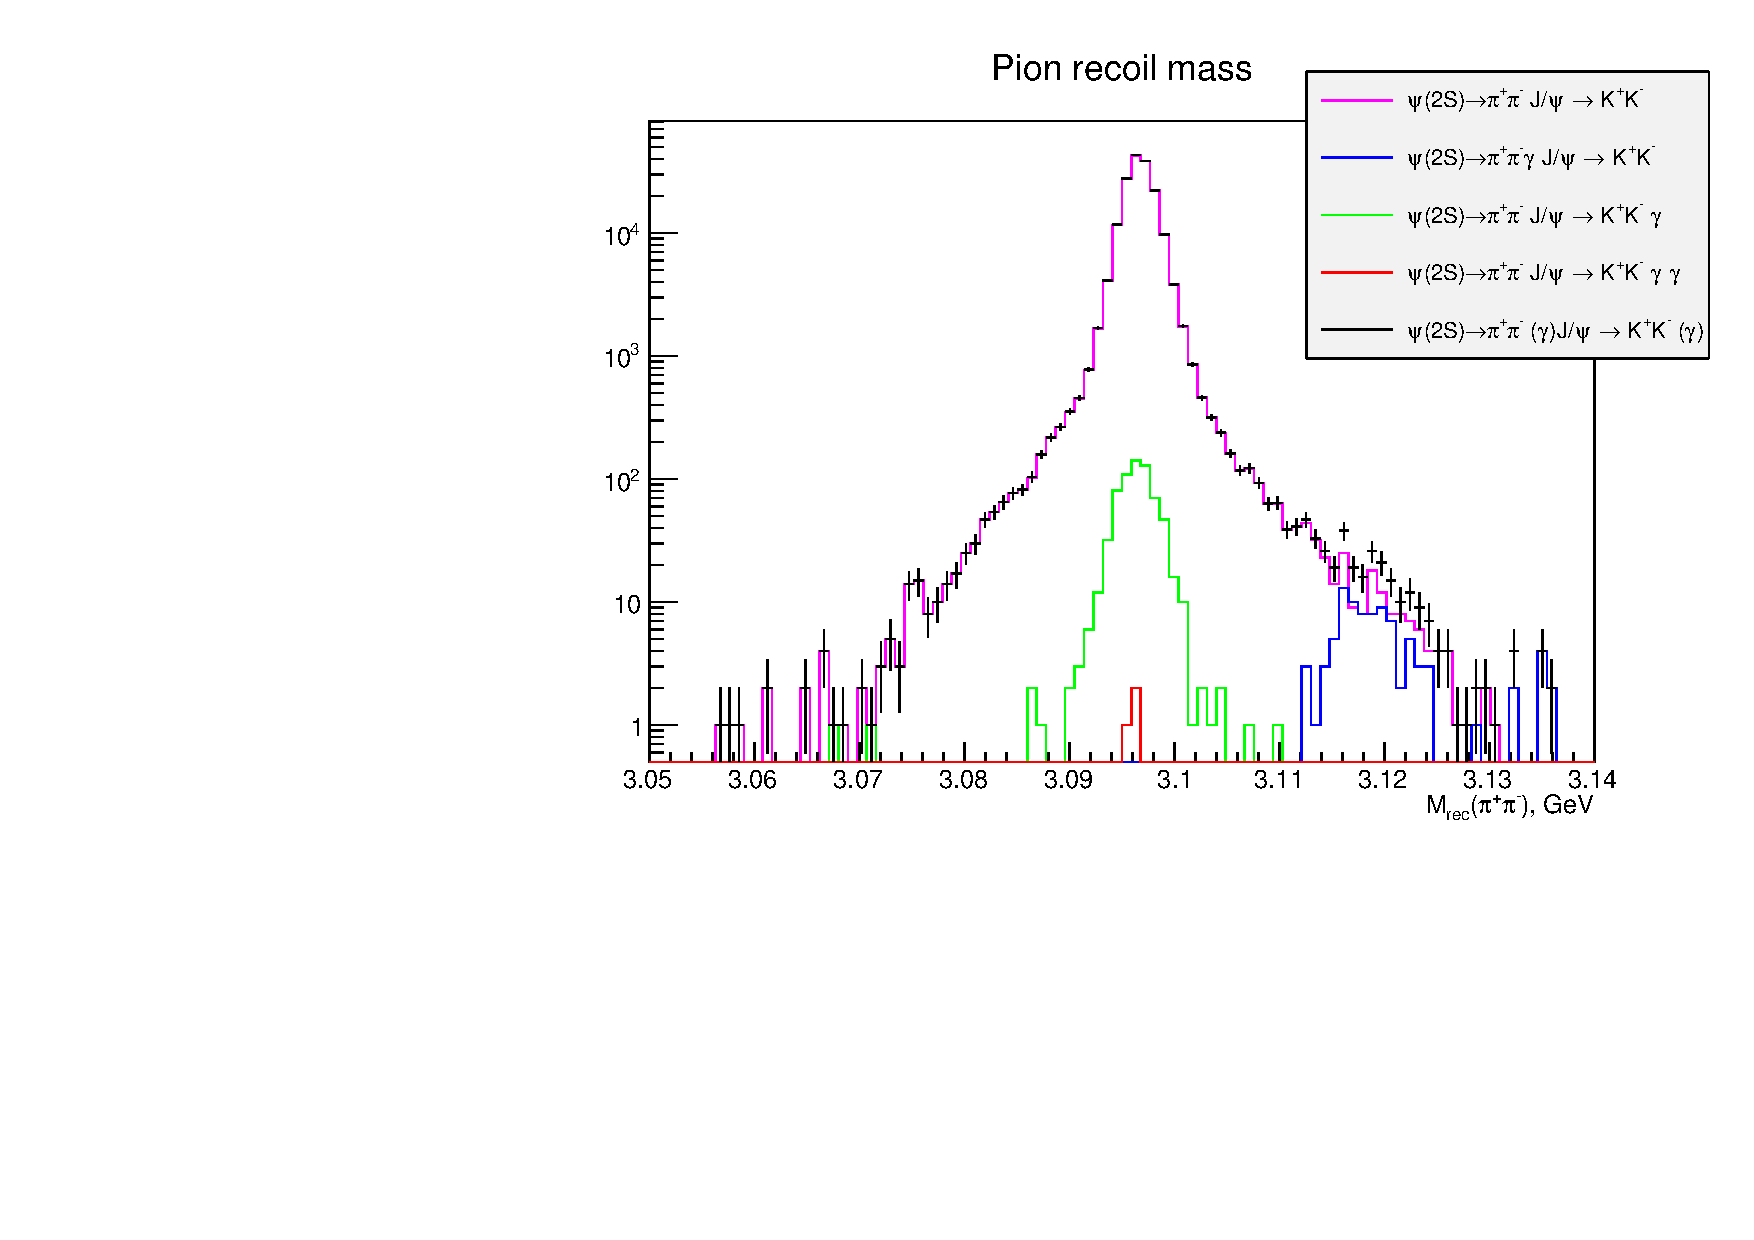
\includegraphics[width=0.9\textwidth]{fig/pion_recoil_radcor.pdf} \hfill
\end{figure}
\end{block}
\end{frame}

\begin{frame}
	\small
\begin{table}
  \centering
  \label{tab:res09}
  \caption{Selection result}
  \begin{tabular}{lll} 
                          & Monte Carlo 2009 & data 2009      \\  \hline
  $ N_{tot}^{KK}$         & 3384             &    3747        \\            
  $ N_{fit}^{KK}$         & $2840\pm65$      &    $3586\pm60$ \\
  $ N_{bg}^{KK}$          & $544\pm23$       &          $161 \pm 13$   \\
  $ N_{tot}^{\mu\mu}$     & $676294$         &       659534   \\
  $ N_{fit}^{\mu\mu}$     & $676294\pm822$   &       $659534 \pm 812$   \\
  $ N_{bg}^{\mu\mu}$      & $0           $   &       0    \\
  $ N_{fit}^{KK}/N_{fit}^{\mu\mu}$& $(4.20 \pm 0.09)\times10^{-3} $ & $(5.44 \pm 0.09)\times 10^{-3}$  \\
  $\varepsilon_{KK}/\varepsilon_{\mu\mu}$ & $1.063 \pm 0.002$ &  $1.063 \pm 0.002$  \\
  $ B_{KK}/B_{\mu\mu}(meas)$   & $(3.95 \pm 0.09)\times 10^{-3}$  & $(5.12 \pm 0.09)\times 10^{-3}$ \\
  $ B_{KK}/B_{\mu\mu}(set\,  in\,  MC)$   & $4.00\times 10^{-3}$  &  	\\ 
  $ B_{KK}/B_{\mu\mu}(PDG-2014)$   &                  & $(4.53 \pm 0.29)\times 10^{-3}$ \\
		$ B_{KK}/B_{\mu\mu}(BES)$   &                  &  $(5.08 \pm 0.12)\times 10^{-3}$ \\
\end{tabular}
\end{table}

\end{frame}


\section{Итерференция}
\begin{frame}

\begin{figure}
\begin{center}
  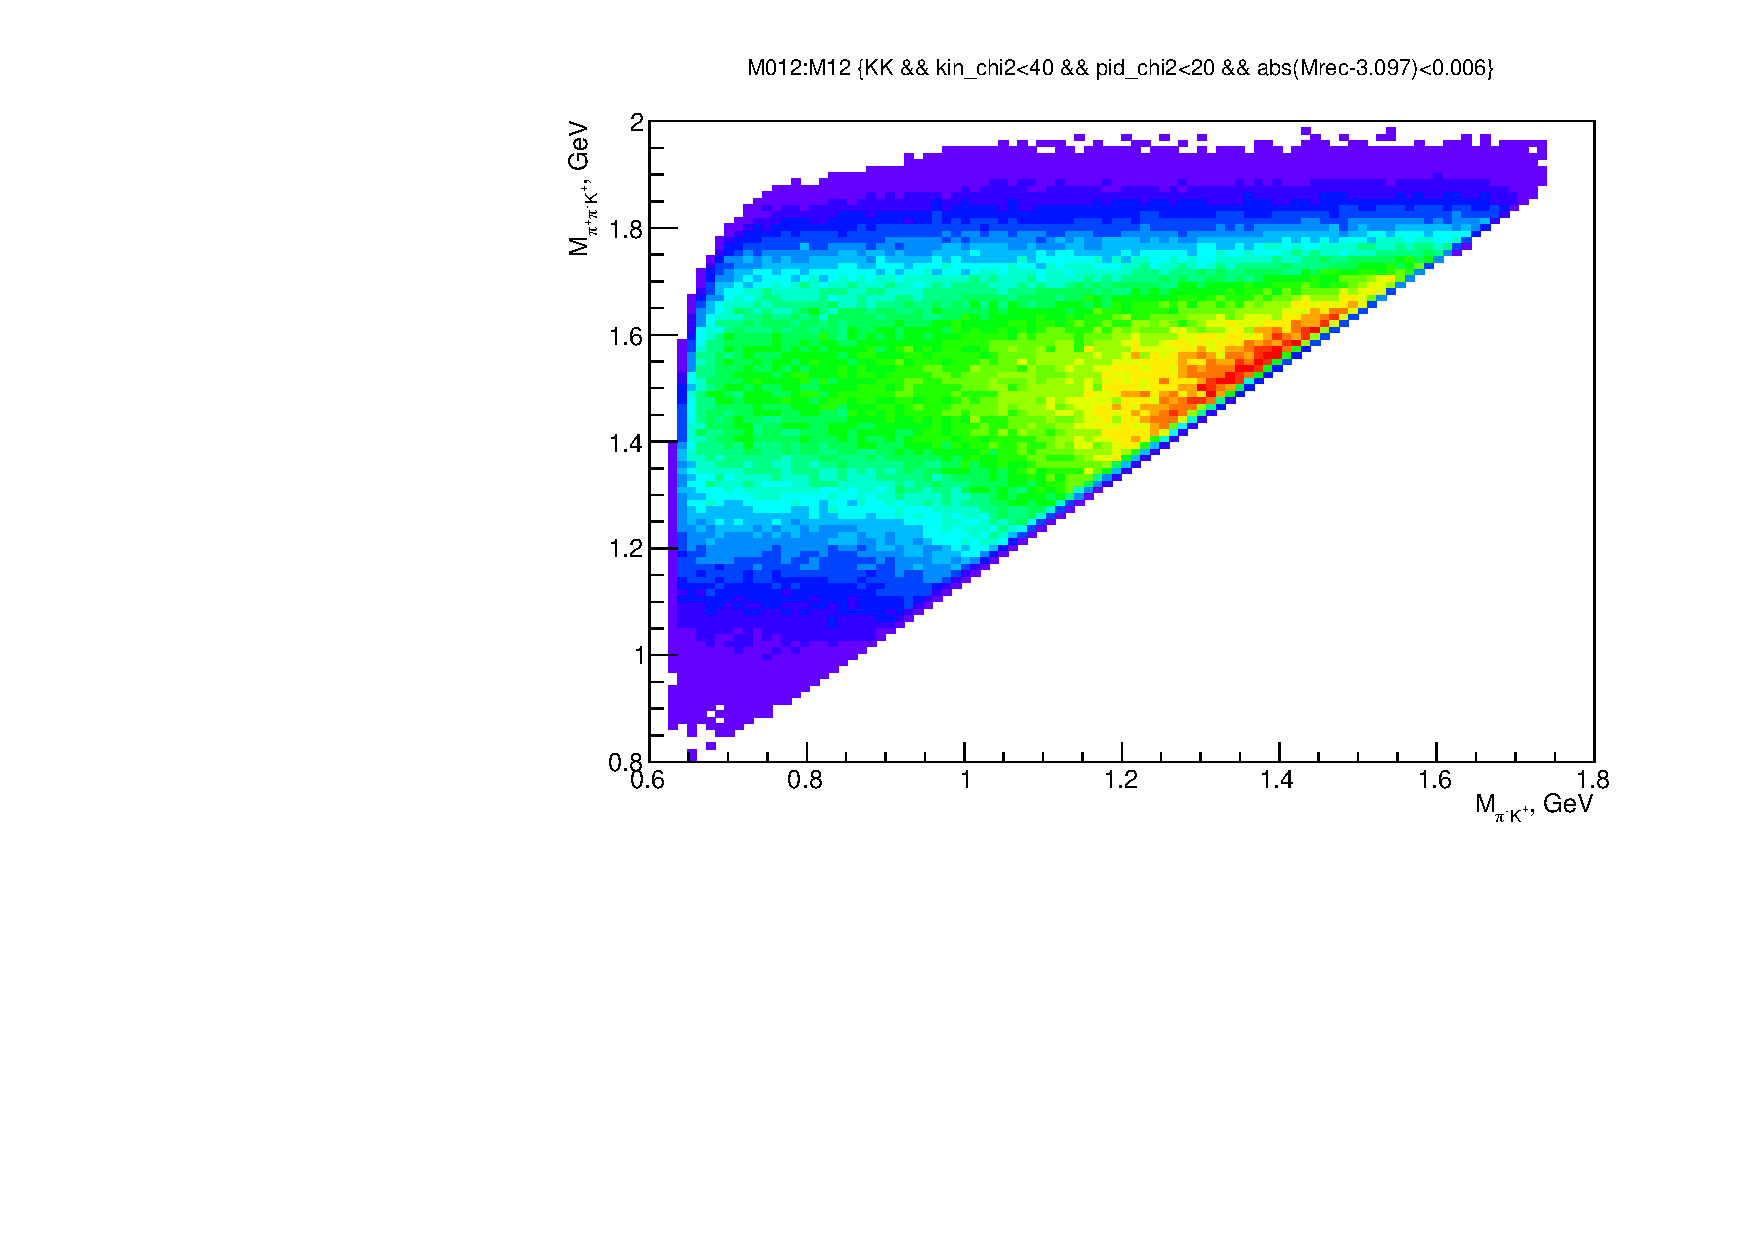
\includegraphics[width=0.5\textwidth]{fig/dalitz-KK2.pdf}
  \hfill
  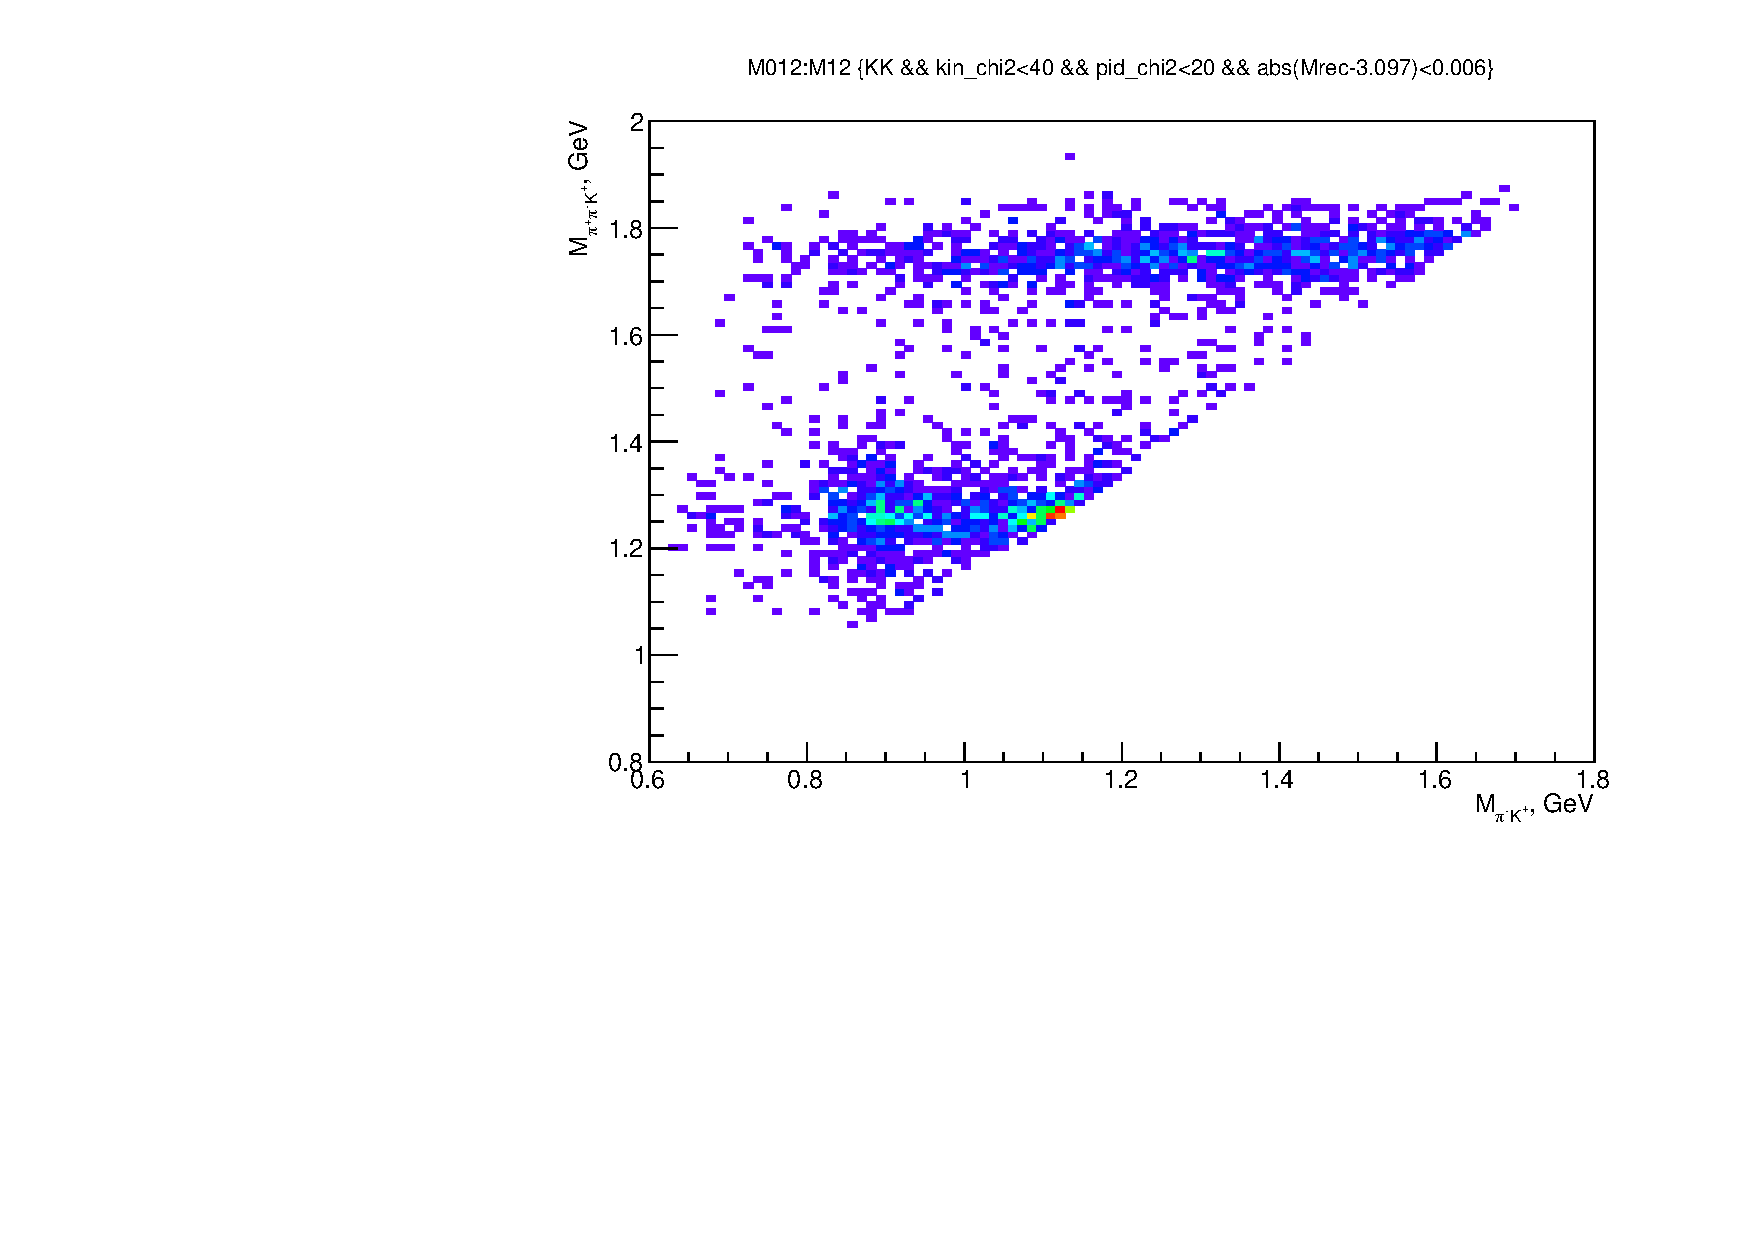
\includegraphics[width=0.5\textwidth]{fig/dalitz-bg2.pdf}
	\caption{Далиц-плот по инвариантной массе $K\pi\pi$ (ось Y), $K\pi$ (ось X) для сигнала (слева) и фона от K1(1270) (справа) }
\end{center}
\end{figure}

\end{frame}

\begin{frame}
	\small
\begin{eqnarray}
  dN_{sig} & = & \epsilon L \sigma_{\psi(2S)} |A(x, y) BW(W)|^2  dW dx dy \\
  dN_{bg} & = & \epsilon L \sigma_{\psi(2S)}  |B(x, y)|^2  dW dx dy,
\end{eqnarray}

here BW(x) is Breight-Wigner function:
\begin{equation}
  BW(W) =  \frac{M \Gamma}{M^2-W^2 - iM\Gamma};
\end{equation}
\begin{eqnarray}
W & = & M_{rec} = \sqrt{(P_{\pi^+}+ P_{\pi^-})^2}, \nonumber \\
x & = & M_{\pipi K^+} = \sqrt{(P_{\pi^+}+ P_{\pi^-} + P_{K^+})^2}, \nonumber \\ 
y & = & M_{\pi^- K^+} = \sqrt{(P_{\pi^-} + P_{K^+})^2}, \nonumber \\
\end{eqnarray}



The interference contribution proportional:
\begin{equation}
	2 |A(x,y) B(x,y) BW(M_{rec}) e^{i\phi}|,
\end{equation}
where $\phi$ is an appropriate phase difference between two amplitudes.


\end{frame}

\begin{frame}
	\tiny
And number of events:
\begin{equation}
  dN_{int} = \epsilon L \sigma_{\psi(2S)} 2\cos(\phi)|A(x,y) B (x,y)|\frac{M \Gamma}{\sqrt{(M^2-W^2)^2 + M^2\Gamma^2}} dW dx dy
\end{equation}


\begin{equation}
  \int_{0}^{\infty}\frac{M^2 \Gamma^2}{(M^2-W^2)^2 + M^2\Gamma^2} dW = \frac{\pi}{2} \Gamma
\end{equation}


\begin{equation}
N_{int} = \epsilon L \sigma_{\psi(2S)} 2\sin(\phi) \Gamma \frac{\pi}{2}\int |A(x,y) B (x,y)|dxdy
\end{equation}
\begin{equation}
  N_{sig} = \epsilon L \sigma_{\psi(2S)} \frac{\pi}{2} \Gamma \int |A(x,y)|^2 dxdy
\end{equation}
\begin{equation}
  N_{bg} = \epsilon L \sigma_{\psi(2S)} \Delta W \int |B(x,y)|^2 dxdy
\end{equation}

\begin{equation}
  \frac{N_{int}}{N_{sig}} = 2\sin\phi
  \sqrt{\frac{N_{bg}}{N_{sig}}\frac{\pi \Gamma}{2 \Delta W}} 
  \frac{\int |A(x,y) B (x,y)|dxdy}{\int |A(x,y)|^2 dxdy\int |B(x,y)|^2 dxdy}
\end{equation}
\end{frame}

\begin{frame}
	\small
Using Monte Carlo for background $\psi(2S) \to K_1(1270) X \to \pipi KK $ and for the signal $\psi(2S) \to J/\psi\pipi \to \pipi KK $ one can receive:
\begin{equation}
  \frac{\int |A(x,y) B (x,y)|dxdy}{\int |A(x,y)|^2 dxdy\int |B(x,y)|^2 dxdy} \approx 0.5
\end{equation}

Then fraction of interference
\begin{equation}
  \frac{N_{int}}{N_{sig}} \le 2 \cdot 0.5 
    \sqrt{\frac{N_{bg}}{N_{sig}}\frac{\pi \Gamma}{2 \Delta W}}   \approx 0.006
\end{equation}
here $\Gamma = \Gamma_{J/\psi} = 0.093$~MeV, $M= M_{J/\psi}=3097$~MeV, $N_{bg}=160$, $N_{sig} = 3586$, $\Delta W = 90$~MeV 
\end{frame}



\section{Планы}

\begin{frame}
	\frametitle{Ближайшие планы}
	\begin{itemize}
		\item Обработать 2012 год.
		\item Обработать континуум на 2E=3.65 GeV
		\item Полное моделирование фона от распадов $\psi(2S)$
		\item ISR фон.
		\item Исследовать систематику в эффективности регистрации.
	\end{itemize}
\end{frame}

\end{document}
